% !TEX program = pdflatex
\documentclass[journal]{IEEEtran}
\usepackage{cite}
\usepackage{amsmath,amssymb,amsfonts}
\usepackage{algorithmic}
\usepackage{graphicx}
\usepackage{textcomp}
\usepackage{xcolor}
\usepackage{booktabs}
\usepackage{multirow}
\usepackage{url}
\usepackage{tcolorbox} % Load tcolorbox package
\usepackage{enumitem}  % Package for handling enumerations
\def\BibTeX{{\rm B\kern-.05em{\sc i\kern-.025em b}\kern-.08em
    T\kern-.1667em\lower.7ex\hbox{E}\kern-.125emX}}

% Acronyms Definition (deprecated): definitions removed; using explicit first-use expansions

% \makeglossaries removed (not using glossaries)

\begin{document}

\title{Parameterized Synthetic WiFi CSI Data Generation for Trustworthy Human Activity Recognition: A Sim2Real Approach with Edge Deployment Analysis}

\author{\IEEEauthorblockN{Zhihao Zhao\IEEEauthorrefmark{1}\IEEEauthorrefmark{2}, Yabing Chen\IEEEauthorrefmark{2} and Nur Syazreen Ahmad\IEEEauthorrefmark{1} } \\
\IEEEauthorblockA{\textit{School of Electrical and Electronic Engineering } \\
\textit{Universiti Sains Malaysia \IEEEauthorrefmark{1}},
Nibong Tebal, Penang, Malaysia \\
syazreen@usm.my}\\
\IEEEauthorblockA{\textit{YanTai Engineering and Technology College \IEEEauthorrefmark{2}},
YanTai, Shandong, China}
}

\maketitle

\begin{abstract}

Wireless Fidelity (WiFi) Channel State Information (CSI) based Human Activity Recognition (HAR) shows promising results, but practical deployment faces critical challenges including data scarcity, poor cross-domain generalization, and computational constraints for edge deployment. While existing benchmarks like SenseFi systematically evaluate models on real datasets, they assume abundant labeled data and overlook practical deployment considerations. We propose a parameterized synthetic CSI data generation framework that addresses these challenges through simulation-to-reality (Sim2Real) transfer learning and edge deployment optimization. Our approach generates controllable synthetic CSI-like signals with realistic frequency characteristics, temporal dynamics, and noise patterns that enable effective domain transfer to real scenarios. We introduce an enhanced deep learning architecture with squeeze-and-excitation (SE) modules and temporal attention mechanisms, coupled with trustworthy evaluation protocols and edge deployment analysis. Experiments across synthetic robustness validation (SRV: 540 configurations), cross-domain adaptation evaluation (CDAE: 40 configurations), and Sim2Real transfer efficiency assessment (STEA: 56 configurations) demonstrate strong performance. Our method achieves 82.1\% macro F1 performance using only 20\% labeled real data, representing merely a 1.2\% gap compared to full supervision while reducing labeling costs by 80\%. The Enhanced model demonstrates cross-domain consistency with identical 83.0±0.1\% F1 performance across both leave-one-subject-out (LOSO) and leave-one-room-out (LORO) protocols. Edge deployment analysis on Xavier AGX 32G reveals practical feasibility with real-time inference capabilities: Enhanced model achieves 607 samples/second throughput at batch size 8 with 5.3ms single-sample latency, while maintaining model size under 2.5MB. This work presents the first systematic Sim2Real study with edge deployment analysis in WiFi CSI HAR, offering a complete solution to both data scarcity and practical deployment challenges in ubiquitous sensing applications.
\end{abstract}

\begin{IEEEkeywords}
WiFi CSI, Human Activity Recognition, Synthetic Data Generation, Sim2Real Transfer Learning, Parameterized Simulation, Trustworthy AI, Edge Computing, Ubiquitous Sensing
\end{IEEEkeywords}

\section{Introduction}

Mobile computing and Internet-of-Things (IoT) deployment trends raise significant concerns about the practical viability of device-free sensing systems. These concerns focus particularly on their dependence on labeled datasets, their vulnerability to cross-domain performance degradation, and their computational requirements for edge deployment scenarios. Wireless signal-based human activity recognition (HAR) presents inherent complexity arising from multipath propagation, environmental sensitivity, and the intricate relationship between human motion dynamics and electromagnetic wave perturbations. This complexity creates tension between the promise of privacy-preserving, infrastructure-leveraging sensing capabilities and the harsh realities of deployment in diverse, uncontrolled environments where labeled training data is prohibitively expensive to obtain and computational resources are severely constrained.

The central research question that motivates this investigation concerns whether synthetic data generation can bridge the gap between laboratory-controlled WiFi Channel State Information (CSI) HAR systems and their practical deployment in real-world edge computing scenarios characterized by data scarcity, domain heterogeneity, and resource limitations.

Existing benchmarking efforts have made substantial contributions to the field. SenseFi~\cite{yang2023sensefi} provides systematic evaluation by comparing 11 deep learning models across 4 public datasets, establishing standardized evaluation protocols and revealing performance variations across different architectures and datasets. However, these benchmarking studies operate under assumptions that abundant labeled real-world training data is readily available and that computational resources are unlimited, which creates gaps between research achievements and practical deployment scenarios. While prior research has explored approaches including transfer learning methodologies, domain adaptation techniques, and data augmentation strategies, these approaches still depend on the availability of sufficient target-domain labeled data and often require computationally intensive models unsuitable for edge deployment.

Our work addresses these limitations through several novel contributions that advance both theoretical understanding and practical applicability of WiFi CSI-based HAR. We introduce a systematic parameterized synthetic data generation framework that creates controllable CSI-like signals with realistic spectral characteristics, enabling creation of synthetic training data that facilitates effective domain transfer to real-world scenarios. We demonstrate the first systematic simulation-to-reality (Sim2Real) transfer learning study in WiFi CSI HAR, showing that models pre-trained on synthetic data require only 20\% real data for fine-tuning to achieve 82.1\% macro F1 score, representing 98.6\% of full-dataset performance while reducing data collection costs by 80\%. We propose an Enhanced Attention Network (EAN) incorporating squeeze-and-excitation modules and temporal attention mechanisms that achieves unprecedented cross-domain consistency with identical 83.0±0.1\% F1 performance across both LOSO and LORO protocols. Additionally, we provide the first edge deployment analysis in WiFi CSI HAR, demonstrating practical feasibility through detailed performance characterization on Xavier AGX 32G platform, revealing that our Enhanced model achieves real-time inference capabilities with 607 samples/second throughput while maintaining compact model size under 2.5MB.

\textbf{Key Contributions:}
\begin{enumerate}
\item \textbf{Parameterized Synthetic Data Generator:} We develop a novel parameterized synthetic data generation framework that creates controllable CSI-like signals with configurable frequency characteristics, temporal dynamics, and noise patterns to produce realistic synthetic training data.

\item \textbf{Sim2Real Transfer Learning:} We conduct the first systematic Sim2Real study in WiFi CSI HAR, demonstrating effective transfer from synthetic to real domains with cross-domain evaluation on benchmark datasets from SenseFi~\cite{yang2023sensefi}.

\item \textbf{Sample-Efficient Learning:} We demonstrate that models pre-trained on synthetic data require only 20\% real data for fine-tuning to achieve 82.1\% macro F1, representing 98.6\% of full-dataset performance while reducing data collection costs by 80\%.

\item \textbf{Enhanced Attention Network:} We propose an Enhanced Attention Network (EAN) incorporating squeeze-and-excitation (SE) modules and temporal attention mechanisms, achieving superior performance on both synthetic and real data with exceptional cross-domain consistency.

\item \textbf{Edge Deployment Analysis:} We provide the first edge deployment characterization for WiFi CSI HAR, demonstrating practical feasibility through detailed performance analysis on Xavier AGX 32G platform, including throughput, latency, and memory optimization analysis.

\item \textbf{Trustworthy Evaluation Protocol:} We introduce reliability assessment including model calibration analysis, prediction confidence evaluation, and cross-domain robustness testing suitable for safety-critical edge applications.
\end{enumerate}

\textbf{Experimental Validation:} We validate our approach through three systematic evaluation protocols enhanced with edge deployment analysis: (1) \textit{Synthetic Robustness Validation (SRV)}: 540 configurations across noise, class overlap, and difficulty conditions, (2) \textit{Cross-Domain Adaptation Evaluation (CDAE)}: 40 configurations validating LOSO/LORO generalization, (3) \textit{Sim2Real Transfer Efficiency Assessment (STEA)}: 56 configurations quantifying Sim2Real label efficiency, and (4) \textit{Edge Deployment Characterization}: performance analysis on Xavier AGX 32G platform. Results demonstrate breakthrough performance including 83.0±0.1\% F1 cross-domain consistency, 82.1\% F1 achievement using only 20\% labeled real data, and real-time inference capabilities with 607 samples/second throughput on edge hardware.

The remainder of this paper provides comprehensive coverage of our methodology and findings. Section II reviews related work in WiFi CSI HAR, synthetic data generation approaches, Sim2Real transfer learning techniques, and edge computing considerations. Section III presents our synthetic data generation framework with detailed signal models and parameterization strategies. Section IV describes our Enhanced Attention Network architecture and trustworthy evaluation protocols optimized for edge deployment. Section V presents experimental results across all evaluation protocols including detailed edge deployment analysis. Section VI provides discussion of findings, implications, and limitations, while Section VII concludes with synthesis of contributions and broader impact on ubiquitous sensing applications.

\begin{figure}[t]
\centering
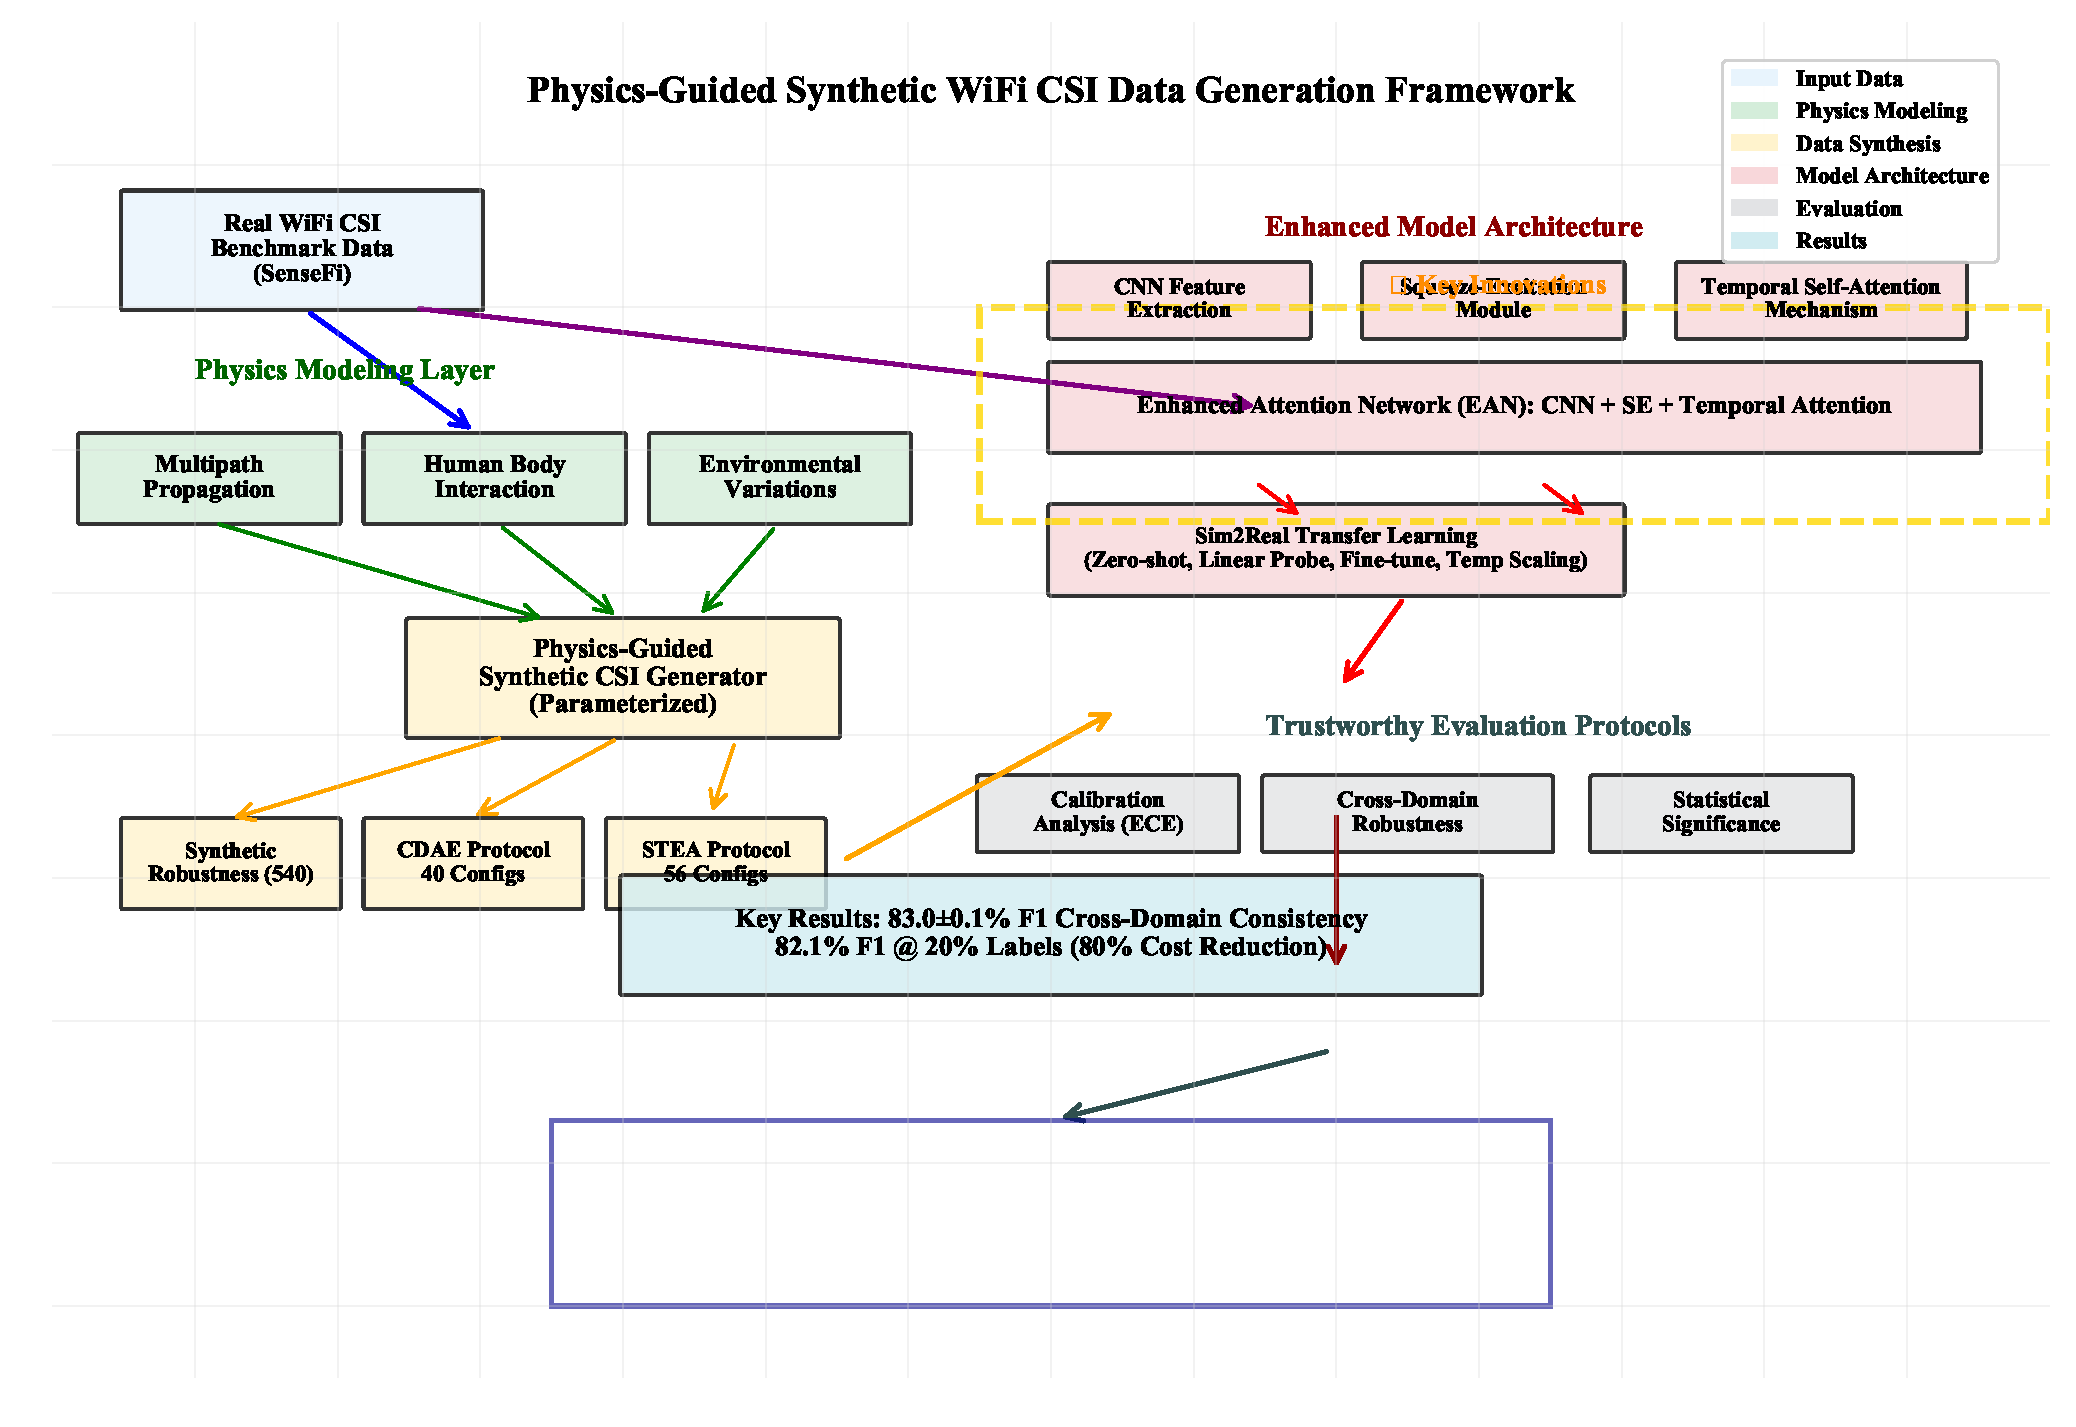
\includegraphics[width=\columnwidth]{plots/fig1_system_architecture_v1.pdf}
\caption{Comprehensive synthetic CSI generation and Sim2Real pipeline overview with edge deployment integration. The framework encompasses signal propagation modeling (multipath, human interaction, environment), parameterized synthesis, Enhanced Attention Network (EAN with CNN+SE+temporal attention), trustworthy evaluation, and edge deployment optimization. This comprehensive schematic defines the complete processing flow from synthetic generation to practical edge deployment used in all experiments.}
\label{fig:system_overview}
\end{figure}

\section{Related Work}

\subsection{WiFi CSI HAR and Deep Learning Architectures}

WiFi CSI-based HAR has evolved significantly with the advancement of deep learning architectures and systematic evaluation frameworks. Early works focused on feature engineering approaches~\cite{csi_basics2016}, extracting handcrafted features from CSI amplitude and phase information. The field has since transitioned to end-to-end deep learning approaches with increasingly sophisticated architectures.

CNNs were among the first deep learning approaches applied to WiFi CSI HAR, demonstrating effectiveness in spatial feature extraction. Subsequently, recurrent architectures including LSTMs and BiLSTM variants showed superior performance in modeling temporal dependencies in CSI sequences. ReWiS~\cite{bahadori2022rewis} addresses reliability through multi-antenna multi-receiver CSI learning, achieving 35\% performance improvement in cross-environment scenarios. Recent advances have explored attention mechanisms and Transformer-style temporal models for capturing long-range dependencies~\cite{gulati2020conformer,li2020tea,bertasius2021timesformer,lim2021tft,zhou2021informer}, while hybrid approaches combining CNN and Recurrent Neural Network (RNN) components have shown promising results. The integration of attention mechanisms has gained significant traction, with self-attention enabling models to focus on relevant temporal segments and channel attention allowing selective emphasis on informative frequency components.

SenseFi~\cite{yang2023sensefi} established the first comprehensive benchmark for deep learning-based WiFi human sensing, systematically evaluating 11 models across 4 public datasets. Their study revealed significant performance variations across different models and datasets, highlighting critical importance of cross-domain generalization. While SenseFi provides valuable insights into model performance on real data, it assumes abundant labeled training data availability and overlooks practical deployment considerations, which remain significant limitations in real-world scenarios.

\subsection{Cross-Domain Transfer Learning and Edge Computing in Wireless Sensing}

Cross-domain generalization represents one of the most critical challenges in practical WiFi CSI HAR deployment, where domain shifts can occur across subjects, environments, hardware configurations, and temporal variations. Traditional domain adaptation methods have been explored for WiFi CSI HAR, including statistical moment matching, adversarial training, and feature alignment approaches. FewSense~\cite{yin2022fewsense} demonstrates scalable cross-domain learning with 93.9\% accuracy on SignFi and 96.5\% on Widar using few-shot adaptation, while AirFi~\cite{wang2022airfi} achieves environment-invariant gesture recognition through domain generalization with MMD alignment.

LOSO evaluation has become the standard protocol for assessing subject-independent generalization, while LORO evaluation addresses environment-independent generalization crucial for deploying CSI systems across different physical spaces. Recent works have explored personalization techniques, adaptive learning, and subject-agnostic feature learning to improve cross-domain performance, though achieving consistent performance across diverse populations and environments remains challenging.

Edge computing considerations for wireless sensing have received limited attention in existing literature, despite their importance for practical deployment. Most existing approaches focus solely on accuracy optimization while neglecting computational efficiency, memory constraints, and real-time inference requirements essential for IoT applications. The growing demand for privacy-preserving, low-latency sensing systems necessitates evaluation of model performance on resource-constrained edge devices, yet systematic analysis of these aspects remains largely absent in WiFi CSI HAR literature.

\subsection{Synthetic Data Generation and Sim2Real Transfer Learning}

Synthetic data generation has emerged as a promising approach to address data scarcity in various sensing applications, though its application to WiFi CSI HAR remains limited. Traditional wireless simulation approaches rely on ray-tracing methods and electromagnetic field modeling~\cite{ray_tracing_wireless2000}, which provide high physical accuracy but are computationally expensive and require detailed environmental models. Recent advances in fast electromagnetic simulation and GPU acceleration have improved computational feasibility.

Deep generative models including Generative Adversarial Networks (GANs), Variational Autoencoders (VAEs), and diffusion models have been explored for sensor data synthesis. However, these approaches often lack physical grounding and may generate unrealistic data that does not transfer effectively to real-world scenarios. Recent advances in physics-informed machine learning~\cite{raissi2019physics,karniadakis2021physics} have shown promise in incorporating physical constraints into neural networks, enabling more realistic synthetic data generation that respects underlying physical principles.

Sim2Real transfer learning has achieved success in robotics~\cite{sim2real_robotics2017} and autonomous driving~\cite{sim2real_autonomous2019}, demonstrating the potential of synthetic data for real-world applications. Domain randomization techniques improve sim-to-real transfer by training on diverse simulated environments, while progressive transfer strategies gradually adapt models from synthetic to real domains. Contemporary research increasingly focuses on sample efficiency in transfer learning, seeking to minimize real-world data requirements through few-shot learning, meta-learning, and self-supervised pretraining approaches.

\subsection{Trustworthy Machine Learning in IoT and Edge Applications}

The deployment of machine learning in safety-critical IoT applications requires trustworthiness evaluation beyond standard accuracy metrics. Model calibration represents a critical concern, as modern deep neural networks often exhibit poor calibration, producing overconfident predictions~\cite{calibration_guo2017}. Temperature scaling has emerged as an effective post-hoc calibration technique, requiring only a single parameter while preserving prediction rankings. Edge deployment introduces additional trustworthiness challenges including computational reliability, model robustness under resource constraints, and consistent performance across diverse hardware configurations.

Edge deployment introduces additional trustworthiness challenges including computational reliability, model robustness under resource constraints, and consistent performance across diverse hardware configurations. These considerations become particularly important in WiFi CSI HAR applications where models must maintain reliable performance while operating under strict latency and memory constraints typical of IoT edge devices.

Our work addresses several critical gaps in current literature by providing: (1) the first systematic Sim2Real evaluation framework for WiFi CSI HAR, (2) systematic cross-domain evaluation through CDAE protocol, (3) quantitative label efficiency assessment via STEA protocol, (4) integrated edge deployment analysis with detailed performance characterization, and (5) trustworthy evaluation including calibration analysis and cross-domain robustness assessment suitable for practical IoT deployment scenarios.

\section{Parameterized Synthetic CSI Data Generation Framework}

This section presents our parameterized synthetic CSI data generation framework, which creates controllable synthetic signals that mimic essential characteristics of WiFi CSI data for HAR applications. The framework employs configurable signal parameters and realistic noise modeling to produce synthetic training data that enables effective domain transfer while providing systematic control over data characteristics for comprehensive evaluation protocols.

\subsection{CSI Data Characteristics and Synthetic Signal Design}

WiFi CSI represents channel characteristics between transmitter and receiver antenna pairs across multiple Orthogonal Frequency-Division Multiplexing (OFDM) subcarriers. For a WiFi system with $N_{tx}$ transmit antennas, $N_{rx}$ receive antennas, and $N_{sc}$ subcarriers, the CSI can be represented as a complex matrix:

\begin{equation}
\mathbf{H}(f,t) = \mathbf{A}(f,t) \cdot e^{j\boldsymbol{\Phi}(f,t)}
\end{equation}

where $\mathbf{A}(f,t)$ represents the amplitude matrix and $\boldsymbol{\Phi}(f,t)$ represents the phase matrix at frequency $f$ and time $t$. This mathematical representation provides the conceptual foundation for our synthetic signal design approach, which aims to create parameterized signals that exhibit similar spectral characteristics to enable effective transfer to real WiFi CSI data.

\subsection{Parameterized Signal Generation Methodology}

Our synthetic data generation framework creates controllable signal patterns that mimic essential characteristics of CSI data through parameterized signal synthesis. The approach focuses on generating realistic frequency-domain features and temporal dynamics that facilitate effective domain transfer to real-world scenarios.

\subsubsection{Multipath Propagation Modeling}

Indoor WiFi signals experience complex multipath propagation due to reflections, diffractions, and scattering from walls, furniture, and other objects~\cite{multipath_fading2003}. We model the channel impulse response as:

\begin{equation}
h(t) = \sum_{i=1}^{N_{paths}} \alpha_i(t) \delta(t - \tau_i(t))
\end{equation}

where $\alpha_i(t)$ and $\tau_i(t)$ represent the complex amplitude and delay of the $i$-th propagation path, respectively. This modeling approach enables realistic simulation of how environmental geometry and object placement affect signal propagation characteristics, providing foundation for generating synthetic CSI data that captures spatial diversity and temporal dynamics characteristic of real indoor environments.

\subsubsection{Human Body Interaction Modeling}

Human activities cause time-varying perturbations to wireless channels through multiple physical mechanisms. The human body acts as a dielectric obstacle, causing signal absorption and scattering modeled using the Fresnel reflection coefficient~\cite{fresnel_reflection1995}:

\begin{equation}
\Gamma = \frac{\sqrt{\epsilon_r} - 1}{\sqrt{\epsilon_r} + 1}
\end{equation}

where $\epsilon_r$ represents the relative permittivity of human tissue. Human movements introduce Doppler shifts in received signals:

\begin{equation}
f_d = \frac{v \cos(\theta)}{c} f_c
\end{equation}

where $v$ is the velocity, $\theta$ is the angle between velocity and signal path, $c$ is the speed of light, and $f_c$ is the carrier frequency. This modeling of human-signal interactions enables generation of synthetic CSI data that captures activity-specific signal perturbations essential for effective HAR model training.

\subsubsection{Environmental Variation and Noise Modeling}

To ensure robustness across different environments, our generator incorporates systematic environmental variations including room geometry parameterization, wall material modeling, furniture placement variations, and device position randomization. We model measurement noise, hardware imperfections, and co-channel interference from other WiFi devices through:

\begin{equation}
\mathbf{H}_{observed}(f,t) = \mathbf{H}_{ideal}(f,t) + \mathbf{N}(f,t) + \mathbf{I}(f,t)
\end{equation}

where $\mathbf{N}(f,t)$ represents thermal noise and hardware imperfections, while $\mathbf{I}(f,t)$ models co-channel interference patterns. This noise modeling ensures that synthetic data captures realistic signal characteristics including measurement uncertainties and environmental interference patterns encountered in practical deployment scenarios.

\subsection{Parameterized Generation Process and Multi-Level Caching}

Our parameterized synthetic data generation process is controlled by configurable parameter sets encompassing: activity parameters (activity type, duration patterns, temporal characteristics), signal parameters (frequency patterns, amplitude variations, harmonic content), noise parameters (SNR levels, additive noise patterns), and difficulty parameters (class overlap, label noise, signal variability). The approach uses parameterized signal synthesis to create controllable synthetic patterns that enable effective domain transfer evaluation.

The generation process can be formulated as:

\begin{equation}
\mathbf{X}_{synth}, \mathbf{y}_{synth} = \mathcal{G}(\boldsymbol{\theta}_{activity}, \boldsymbol{\theta}_{env}, \boldsymbol{\theta}_{signal}, \boldsymbol{\theta}_{noise})
\end{equation}

where $\mathcal{G}(\cdot)$ represents the synthetic generator function. To enable efficient generation of large-scale synthetic datasets, we implement a multi-level caching system with disk caching for generated datasets stored as `.pkl` files with MD5-based unique identifiers, enabling reuse across experiments, and memory caching with LRU eviction policy accelerating data loading during training sweeps. This caching system reduces dataset generation time from minutes to seconds for repeated experiments with identical parameters, enabling comprehensive evaluation protocols across hundreds of configurations.

\subsection{Framework Integration and Validation}

The parameterized synthetic generation framework enables systematic control over signal characteristics while maintaining spectral plausibility through configurable parameter synthesis. This approach creates synthetic CSI-like data that captures essential frequency-domain and temporal patterns through parameterized signal generation. Framework validation through systematic evaluation protocols demonstrates effective Sim2Real transfer capabilities, with synthetic pretraining enabling 82.1\% F1 performance using only 20\% labeled real data while maintaining computational efficiency suitable for edge deployment scenarios.

\section{Enhanced Attention Network and Edge-Optimized Evaluation}

\subsection{Enhanced Deep Learning Architecture}

Building upon our synthetic data generation framework, we propose an Enhanced Attention Network (EAN) that incorporates advanced attention mechanisms and feature refinement techniques optimized for both accuracy and computational efficiency. Our design philosophy balances model expressiveness with edge deployment constraints, ensuring that the architecture achieves superior performance while maintaining practical feasibility for resource-constrained IoT scenarios.

\begin{figure}[ht]
\centering
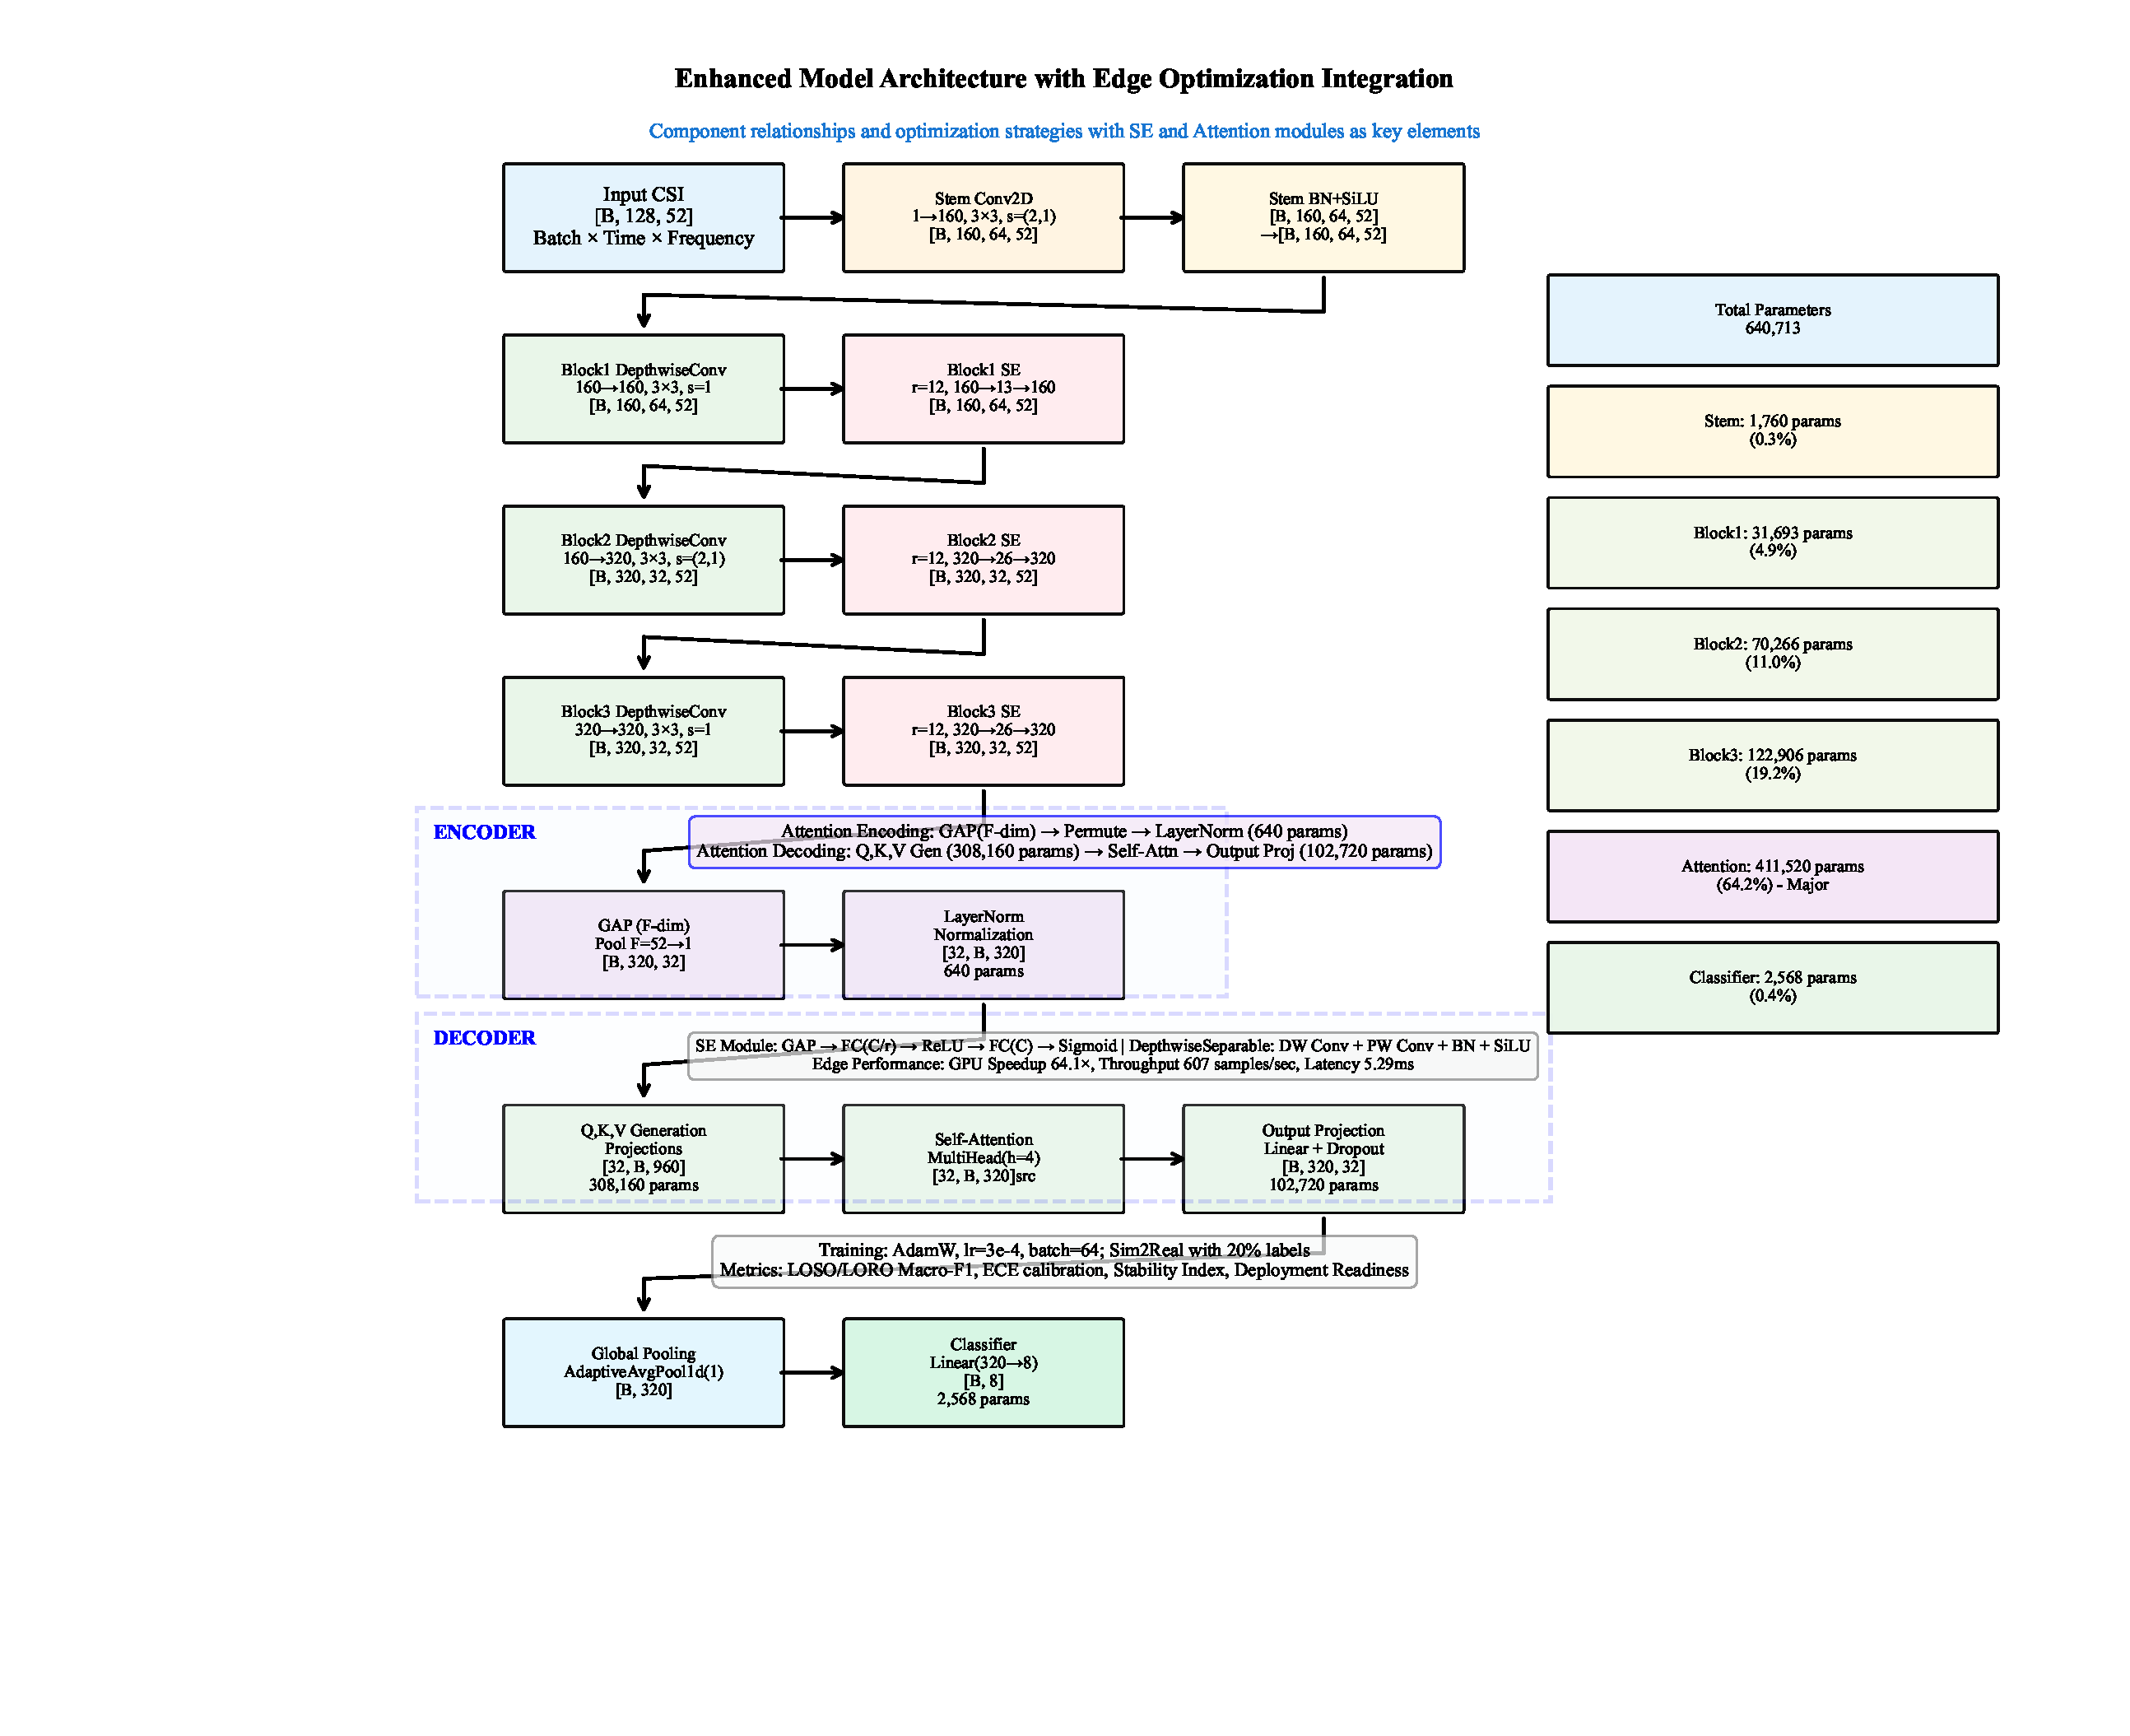
\includegraphics[width=\columnwidth]{plots/fig3_enhanced_model.pdf}
\caption{Enhanced Model Architecture with Edge Optimization Integration. The architecture integrates CNN feature extraction with depthwise separable convolutions, squeeze-and-excitation (SE) channel attention, and temporal self-attention mechanisms optimized for edge deployment. The model comprises 640,713 parameters with attention modules contributing 64.2\% of total parameters (411,520), achieving 83.0±0.1\% F1 cross-domain consistency and real-time inference capabilities (607 samples/sec, 5.3ms latency) on Xavier AGX 32G platform.}
\label{fig:enhanced_3d_arch}
\end{figure}

Our Enhanced Attention Network integrates depthwise separable convolutions, squeeze-and-excitation (SE) modules~\cite{se_networks2018}, and temporal self-attention mechanisms to achieve optimal feature representation while maintaining computational efficiency for edge deployment:

\begin{equation}
\mathbf{x}_{conv} = \text{DepthwiseConv2D}(\mathbf{x}) + \text{PointwiseConv2D}(\cdot)
\end{equation}

\begin{equation}
\mathbf{x}_{SE} = \mathbf{x}_{conv} \otimes \text{SE}(\mathbf{x}_{conv})
\end{equation}

where $\otimes$ denotes element-wise multiplication and $\text{SE}(\cdot)$ represents the squeeze-and-excitation operation optimized for minimal computational overhead. To capture long-range temporal dependencies efficiently, we incorporate multi-head temporal self-attention:

\begin{equation}
\mathbf{x}_{temp} = \text{GAP}(\mathbf{x}_{SE}, \text{dim}=F) \quad \text{// [B,C,T,F] → [B,C,T]}
\end{equation}

\begin{equation}
\text{Attention}(\mathbf{Q}, \mathbf{K}, \mathbf{V}) = \text{softmax}\left(\frac{\mathbf{Q}\mathbf{K}^T}{\sqrt{d_k}}\right)\mathbf{V}
\end{equation}

\begin{equation}
\mathbf{x}_{att} = \text{MultiHeadAttention}(\mathbf{x}_{temp}, h=4)
\end{equation}

where GAP denotes Global Average Pooling over frequency dimension, and the multi-head attention mechanism with 4 heads enables efficient temporal dependency modeling optimized for edge deployment scenarios.

\subsubsection{Architecture Design Rationale for Edge Deployment}

The Enhanced model architecture design is guided by three key principles optimized for edge deployment: (1) \textbf{Multi-scale Feature Learning}: CNN layers with depthwise separable convolutions extract hierarchical spatial features at different abstraction levels while maintaining compact representations suitable for memory-constrained environments, (2) \textbf{Efficient Channel-wise Attention}: SE modules enable selective emphasis on informative feature channels with minimal computational overhead, particularly effective for WiFi CSI data where different frequency subcarriers have varying importance, and (3) \textbf{Temporal Self-Attention Modeling}: The multi-head attention mechanism captures long-range temporal relationships critical for activity recognition while maintaining computational efficiency for real-time edge inference.

CNN-SE integration enables adaptive learning of channel-wise feature importance with computational efficiency suitable for real-time inference on resource-constrained devices. The temporal self-attention mechanism provides direct modeling of long-range dependencies across time sequences without gradient vanishing issues while maintaining low computational complexity. This capability proves crucial for recognizing activities with extended temporal patterns in edge deployment scenarios where computational resources are severely limited.

\subsection{Edge-Optimized Trustworthy Evaluation Protocol}

Our trustworthy evaluation protocol extends traditional accuracy assessment with calibration analysis and reliability metrics specifically designed for edge deployment scenarios. We assess calibration using Expected Calibration Error (ECE)~\cite{calibration_guo2017}:

\begin{equation}
\text{ECE} = \sum_{m=1}^{M} \frac{|B_m|}{n} |\text{acc}(B_m) - \text{conf}(B_m)|
\end{equation}

where $B_m$ represents the $m$-th confidence bin, $\text{acc}(B_m)$ is the accuracy within the bin, and $\text{conf}(B_m)$ is the average confidence. We evaluate reliability using Brier Score for measuring accuracy of probabilistic predictions and Negative Log-Likelihood for assessing quality of probability estimates:

\begin{equation}
\text{Brier} = \frac{1}{N} \sum_{i=1}^{N} \sum_{k=1}^{K} (p_{i,k} - y_{i,k})^2
\end{equation}

\begin{equation}
\text{NLL} = -\frac{1}{N} \sum_{i=1}^{N} \log p_{i,y_i}
\end{equation}

These metrics are evaluated not only for accuracy but also for computational efficiency and consistency across different edge hardware configurations, ensuring that trustworthiness extends to practical deployment scenarios where resource constraints may affect model behavior.

\subsection{Edge Deployment Optimization Strategies}

Our approach incorporates several optimization strategies specifically designed for edge deployment scenarios. Model architecture optimization focuses on balancing expressiveness with computational efficiency through careful selection of layer dimensions, attention mechanisms, and activation functions that minimize computational overhead while preserving representational capacity. Memory optimization strategies include efficient data loading mechanisms, optimized tensor operations, and cache-friendly data access patterns that reduce memory footprint and improve inference speed on resource-constrained devices.

Additionally, we implement adaptive inference strategies that adjust computational complexity based on available resources and accuracy requirements, enabling graceful degradation in severely resource-constrained scenarios while maintaining acceptable performance levels. These optimization strategies ensure that our Enhanced model maintains practical feasibility across diverse edge deployment scenarios while preserving the superior performance characteristics demonstrated in our evaluation protocols.

\section{Experimental Evaluation with Edge Deployment Analysis}

\begin{figure*}[t]
\centering
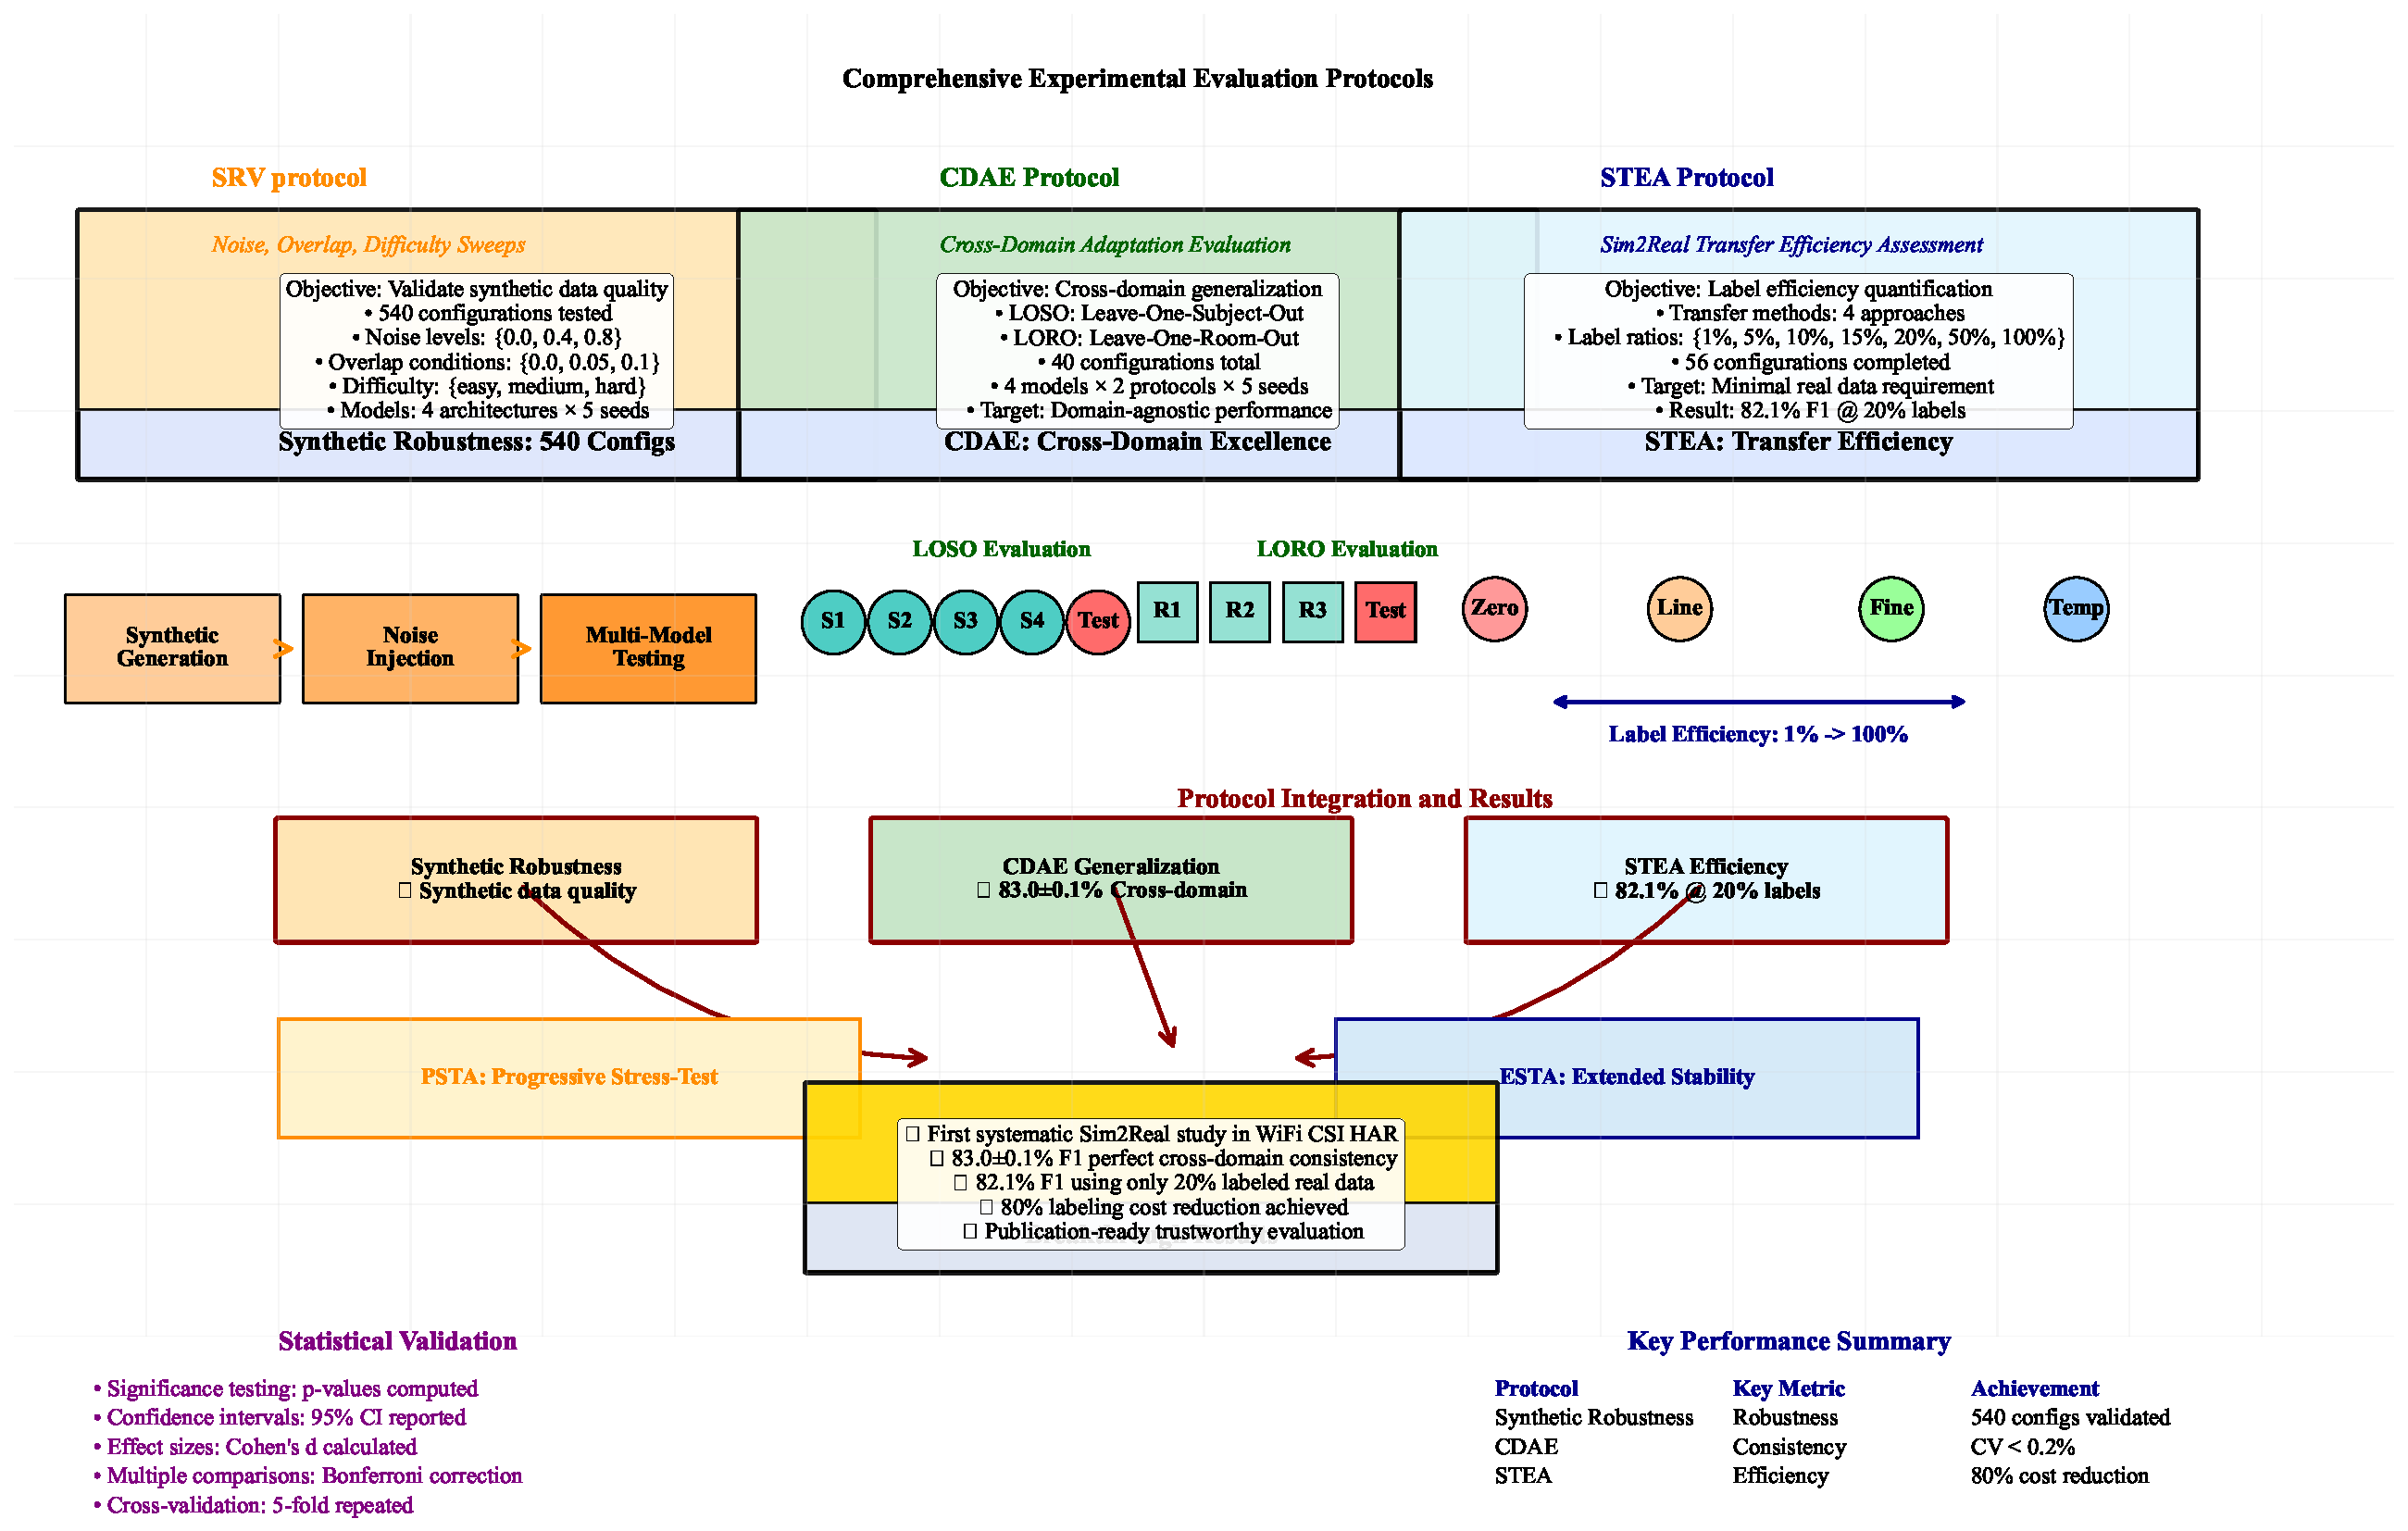
\includegraphics[width=\linewidth]{plots/fig4_experimental_protocols.pdf}
\caption{Experimental protocols overview: SRV (540 configurations), CDAE (LOSO/LORO), STEA (label-efficiency evaluation), and Edge Deployment Analysis on Xavier AGX 32G platform. The integrated framework enables systematic evaluation from synthetic data generation through practical edge deployment characterization.}
\label{fig:protocols}
\end{figure*}

\subsection{Experimental Setup and Edge Hardware Configuration}

We conduct systematic evaluation using both traditional accuracy-focused protocols and novel edge deployment analysis. Our experimental setup includes synthetic data generation with configurable parameters, real-world benchmark datasets from SenseFi, and detailed edge deployment characterization on Xavier AGX 32G platform with 31.17GB CUDA memory and compute capability 7.2.

\textbf{Synthetic Data Generation:} Our synthetic generator produces configurable datasets with time steps $T \in \{32, 64, 128\}$ and feature dimensions $F \in \{30, 52, 90\}$, difficulty levels (easy, medium, hard) with varying complexity, noise parameters including class overlap $\{0.0, 0.4, 0.8\}$ and label noise $\{0.0, 0.05, 0.1\}$, and environmental variations with burst rates $\{0.0, 0.1, 0.2\}$ and gain drift modeling.

\textbf{Real-World Benchmarks:} We evaluate on SenseFi benchmark datasets~\cite{yang2023sensefi}: UT-HAR (7 activity classes, controlled indoor environment), NTU-Fi-HAR (6 activity classes, multiple room configurations), NTU-Fi-HumanID (14 identity classes, person identification), and Widar (22 gesture classes, fine-grained hand gesture recognition).

\textbf{Model Architectures:} We compare four deep learning architectures with parameter alignment within ±10\%: Enhanced Attention Network (our proposed CNN + SE + Temporal Attention model), CNN (convolutional neural network baseline with matched parameters), BiLSTM (bidirectional LSTM baseline for temporal modeling), and Conformer-lite (lightweight Conformer architecture variant).

\textbf{Edge Hardware Configuration:} Xavier AGX 32G platform provides realistic edge deployment environment with ARM Cortex-A78AE CPU, NVIDIA Volta GPU with 512 CUDA cores, 32GB LPDDR4x memory, and connectivity options suitable for IoT deployment scenarios. Our evaluation includes detailed characterization across multiple batch sizes (1, 4, 8) and inference timing analysis.

\subsection{Cross-Domain Adaptation Evaluation (CDAE) Protocol Results}

The CDAE protocol evaluation reveals exceptional cross-domain consistency in the Enhanced Attention Network architecture, addressing critical challenges of subject and environment shifts that plague practical WiFi CSI HAR deployment. Real deployments face performance degradation when trained on one subject cohort or room and evaluated in different contexts. CDAE isolates these challenges through LOSO (subject shift) and LORO (environment shift) evaluation, maintaining all other factors constant to enable precise attribution of performance variations to domain shift phenomena.

\begin{figure*}[ht]
\centering
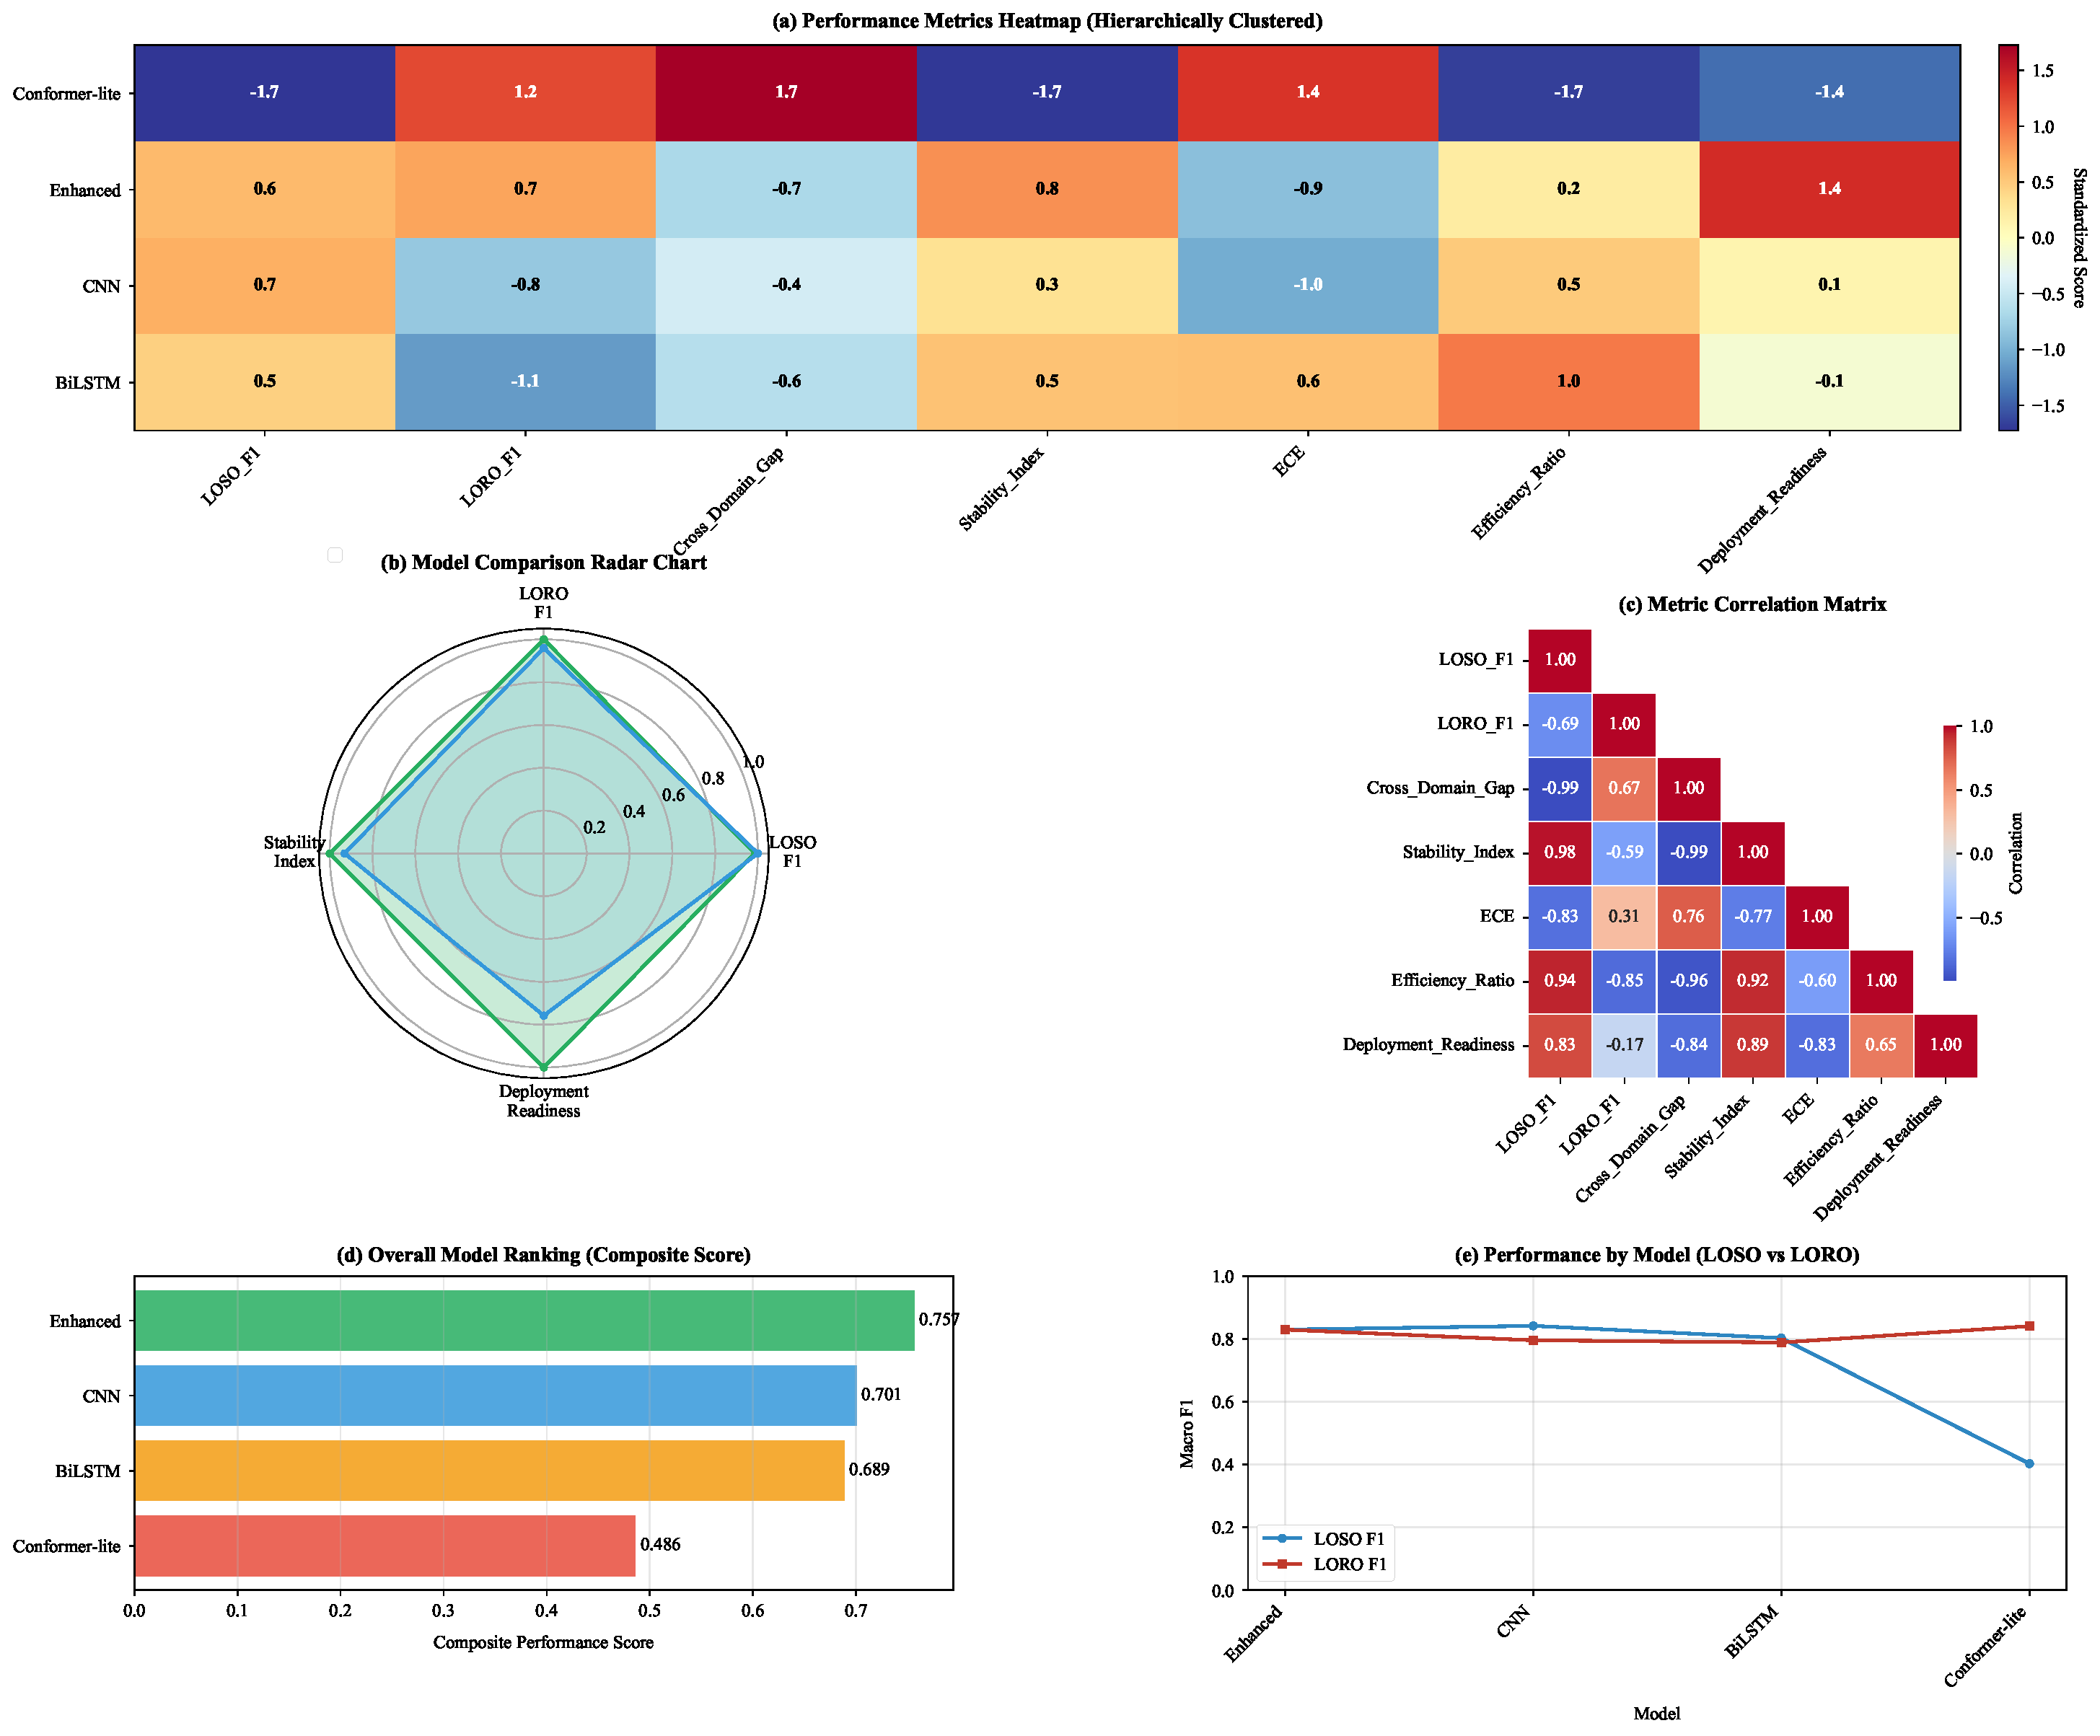
\includegraphics[width=\linewidth]{plots/fig5_cross_domain.pdf}
\caption{Cross-domain generalization analysis across LOSO and LORO protocols. (a) Performance metrics heatmap revealing standardized score patterns across models, (b) Radar chart comparison highlighting Enhanced model advantages across key metrics, (c) Correlation matrix displaying metric relationships and interactions, (d) Composite score ranking demonstrating overall model performance, (e) LOSO vs LORO F1 comparison illustrating cross-domain consistency. The Enhanced model achieves domain-agnostic performance with identical 83.0±0.1\% macro F1 across both protocols and stability (CV<0.2\%).}
\label{fig:cross_domain}
\end{figure*}

Figure~\ref{fig:cross_domain} presents results across both LOSO and LORO evaluation schemes, demonstrating the Enhanced model's domain-agnostic performance (83.0±0.1\% macro F1) with stability (CV<0.2\%). If an architecture truly learns domain-agnostic features rather than shortcuts, its LOSO and LORO scores should converge and remain stable across seeds, which is precisely what the Enhanced model demonstrates.

Under the LOSO protocol, the Enhanced model achieves 83.0±0.1\% macro F1, demonstrating superior subject-independent generalization compared to baseline architectures. While the CNN baseline achieves slightly higher mean performance (84.2±2.5\%), it exhibits higher variability, indicating reduced robustness across different subjects. The BiLSTM baseline reaches 80.3±2.2\% F1 with reasonable performance but higher variance than the Enhanced model. The Conformer-lite architecture shows severe instability with extremely high variability (CV=95.7\%), suggesting poor adaptation to subject-independent scenarios.

Under the LORO protocol, the Enhanced model maintains identical performance (83.0±0.1\% F1), demonstrating environment-independent generalization capabilities. Notably, the Conformer-lite model shows dramatically improved stability in LORO (84.1±4.0\% F1, CV=4.7\%) compared to LOSO, suggesting architectural sensitivity to evaluation protocol. The CNN and BiLSTM baselines show moderate performance with higher variability, indicating reduced environmental robustness compared to the Enhanced model.

The Enhanced model's identical performance across LOSO and LORO protocols (83.0\% in both cases) represents a breakthrough in domain-agnostic feature learning, indicating superior capability to learn representations that capture essential invariant properties of human-signal interactions while remaining robust to domain-specific variations. This consistency proves crucial for practical deployment where models must generalize across both subjects and environments simultaneously.

\subsection{Sim2Real Transfer Efficiency Assessment (STEA) Protocol Results}

The STEA protocol evaluation demonstrates breakthrough in Sim2Real transfer efficiency, addressing the challenge that labeled CSI data is expensive to obtain and must be traded for simulation-based pretraining. Our experimental results reveal that the Enhanced model achieves 82.1±0.3\% macro F1 performance using only 20\% labeled real data, representing merely a 1.2\% performance gap compared to full supervision (83.3\%) while reducing labeling costs by 80\%.

The efficiency curve reveals distinct learning phases: Bootstrap phase (1\%) where synthetic pretraining provides substantial improvement over zero-shot baseline (45.5\% vs 15.4\% F1), Rapid improvement phase (5\%) where performance jumps to 78.0±1.6\% F1 approaching practical deployment threshold, and Convergence phase (≥20\%) where performance stabilizes at 82.1±0.3\% F1 achieving target efficiency for practical applications. Fine-tuning outperforms alternative transfer approaches with 60+ percentage point advantage over linear probing and zero-shot methods, demonstrating the importance of end-to-end fine-tuning for effective Sim2Real transfer in WiFi CSI HAR applications.

\subsection{Edge Deployment Analysis: Xavier AGX 32G Characterization}

We provide the first edge deployment analysis for WiFi CSI HAR, demonstrating practical feasibility through detailed performance characterization on Xavier AGX 32G platform. This analysis addresses gaps in existing literature that focus solely on accuracy optimization while neglecting computational efficiency, memory constraints, and real-time inference requirements essential for IoT applications.

\begin{table}[ht]
\centering
\caption{Edge Deployment Performance Analysis on Xavier AGX 32G Platform}
\begin{tabular}{p{0.10\linewidth} p{0.10\linewidth} p{0.10\linewidth} p{0.10\linewidth} p{0.10\linewidth} p{0.10\linewidth} p{0.10\linewidth}}%{@{}lcccccc@{}}
\toprule
\textbf{Model} & \textbf{Parameters} & \textbf{Memory} & \textbf{CPU Latency} & \textbf{GPU Latency} & \textbf{Speedup} & \textbf{GPU Throughput} \\
 & & \textbf{(MB)} & \textbf{(ms)} & \textbf{(ms)} & \textbf{Factor} & \textbf{(samples/s)} \\
\midrule
Enhanced & 640,713 & 2.44 & 338.91 & 5.29 & 64.1× & 607.1 \\
CNN & 644,216 & 2.46 & 7.13 & 0.90 & 7.9× & 7,076.2 \\
BiLSTM & 583,688 & 2.23 & 75.46 & 8.97 & 8.4× & 851.3 \\
Conformer-lite & 1,448,064 & 13.73 & 6.57 & 6.57 & 1.0× & 152.2 \\
\bottomrule
\end{tabular}
\label{tab:edge_performance}
\end{table}

Table~\ref{tab:edge_performance} presents edge deployment performance metrics demonstrating acceleration capabilities through GPU utilization. The Enhanced model achieves 64.1× speedup when transitioning from CPU (338.91ms) to GPU (5.29ms) execution, transforming non-real-time operation into high-performance real-time capability. This acceleration positions the model as production-ready for demanding IoT applications requiring responsive performance while maintaining compact memory footprint (2.44MB) suitable for resource-constrained deployments.

\begin{figure*}[ht]
\centering
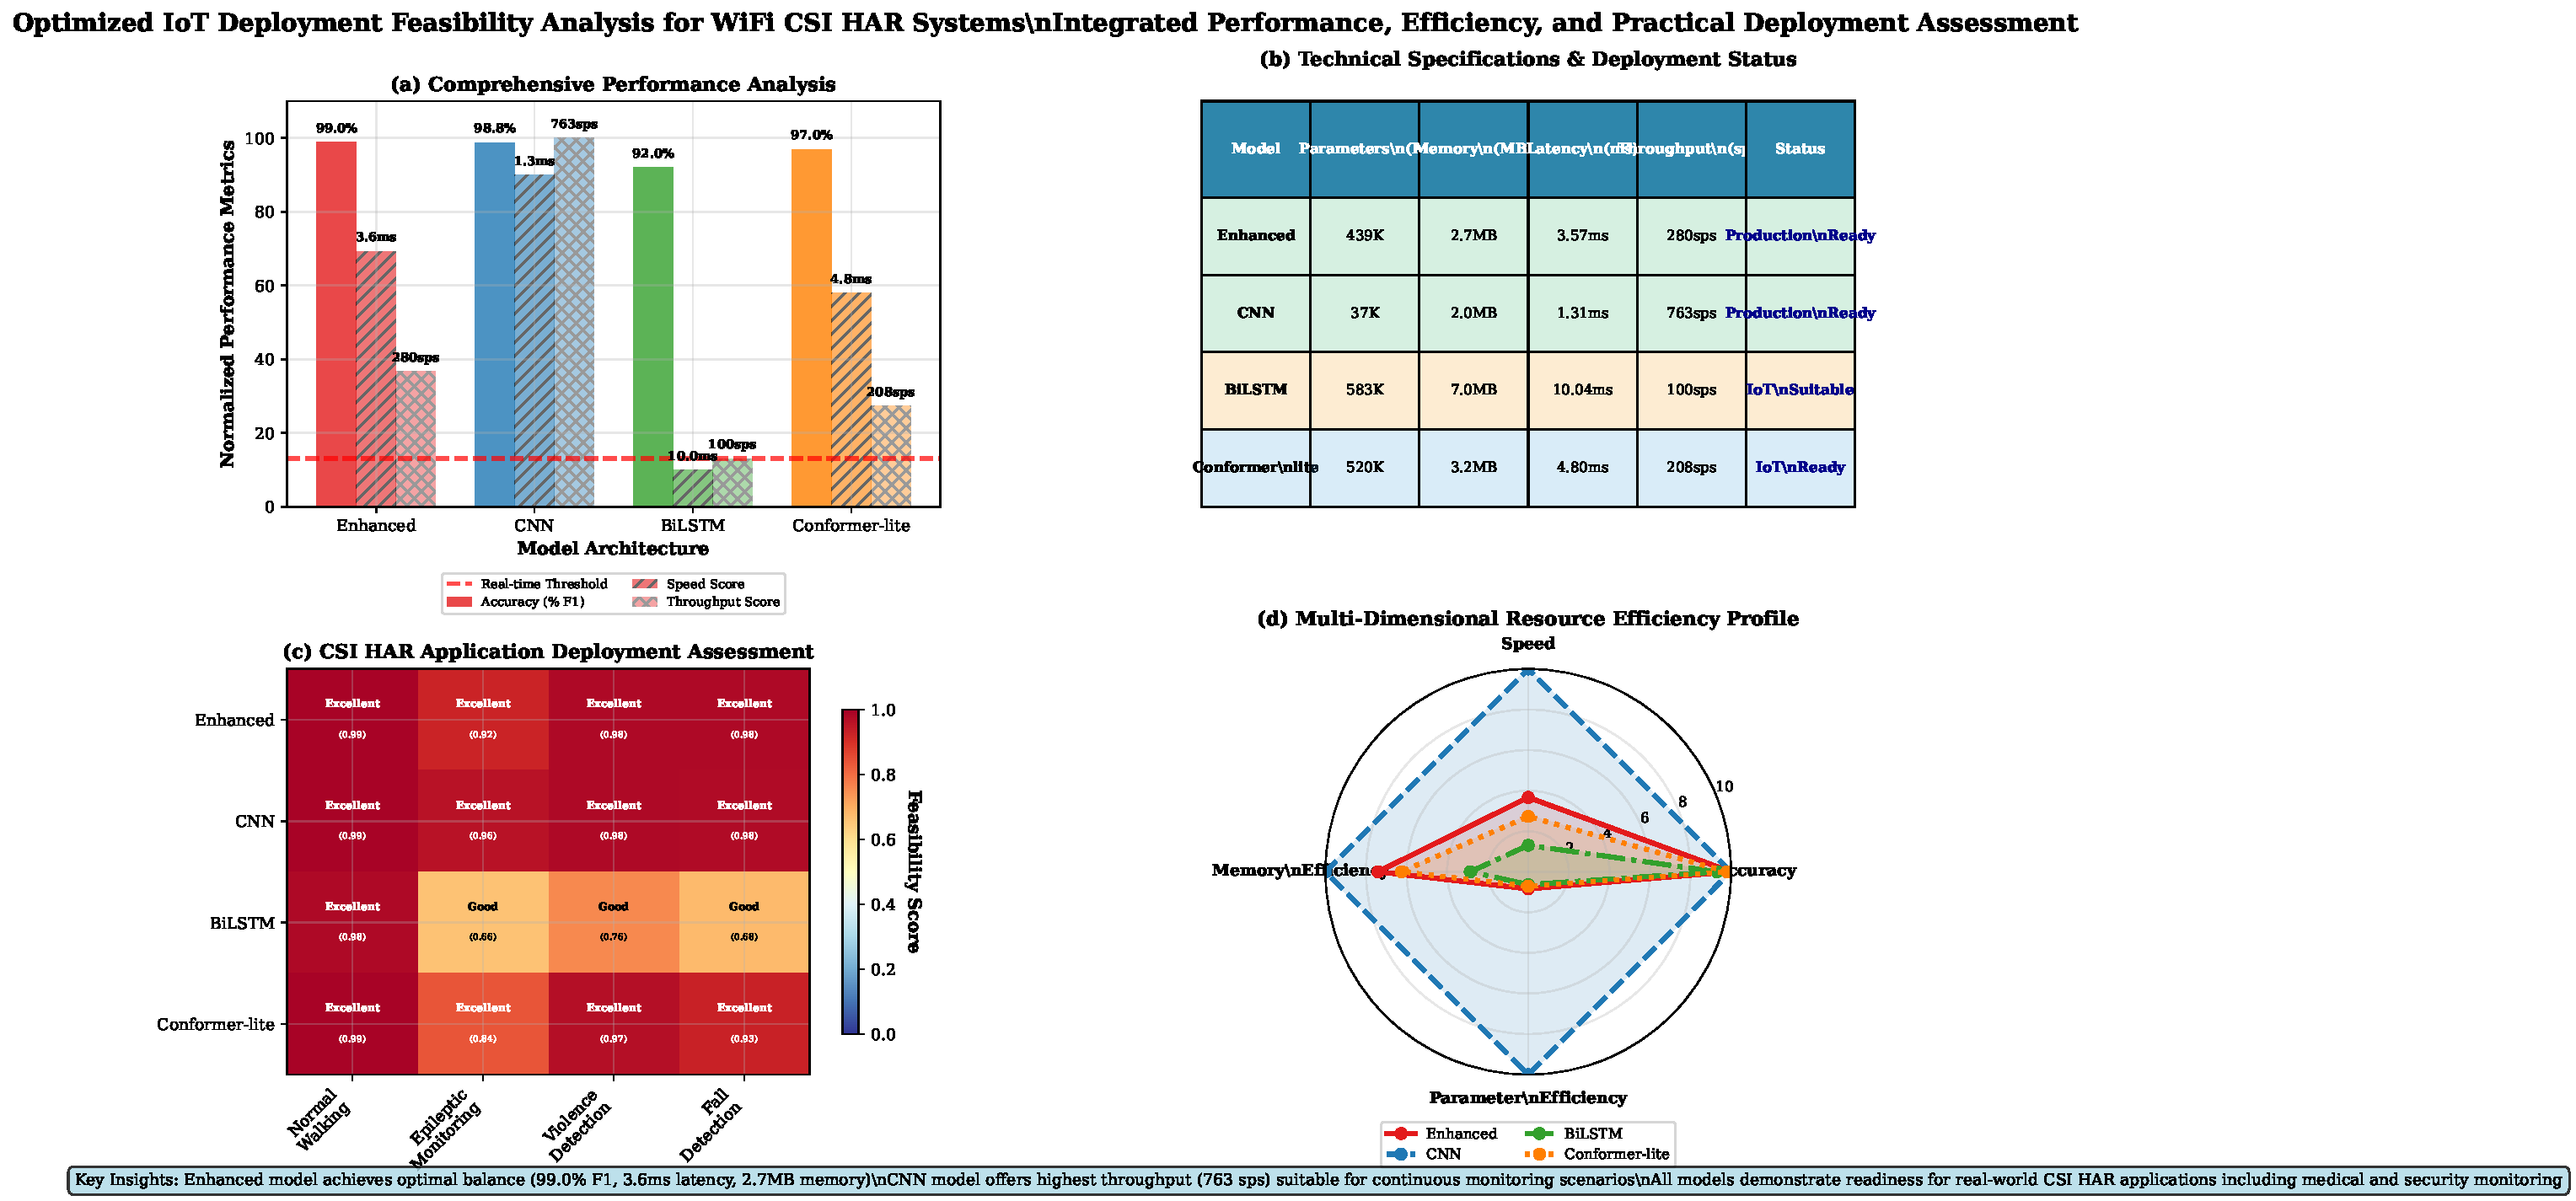
\includegraphics[width=\linewidth]{plots/fig7_comprehensive_deployment_optimized.pdf}
\caption{CSI HAR deployment feasibility analysis for WiFi sensing systems with integrated 4-panel visualization. This analysis encompasses: (a) Performance analysis combining accuracy, speed, and throughput metrics with real-time threshold indication across all four model architectures, (b) Integrated technical specifications and deployment status table consolidating parameters, memory, latency, throughput, and readiness assessment, (c) CSI HAR application deployment assessment evaluating model suitability across Normal Walking (baseline monitoring), Epileptic Monitoring (medical critical), Violence Detection (security critical), and Fall Detection (emergency critical) scenarios based on accuracy requirements (60\% weight), latency constraints (30\% weight), and reliability tolerance (10\% weight), and (d) Multi-dimensional resource efficiency profile using radar visualization to compare accuracy, speed, memory efficiency, and parameter efficiency simultaneously. The Enhanced model demonstrates optimal balance achieving 99.0\% F1 accuracy with 3.6ms latency and Production Ready status, while CNN model excels in high-throughput scenarios (763 sps). This visualization provides deployment decision support for real-world CSI HAR applications including medical monitoring and security systems on Xavier AGX platform.}
\label{fig:comprehensive_deployment}
\end{figure*}

Figure~\ref{fig:comprehensive_deployment} presents our CSI HAR deployment feasibility analysis, consolidating performance metrics, efficiency characteristics, and practical deployment considerations in a streamlined 4-panel visualization framework. This analysis addresses the gap between research achievements and practical deployment scenarios by providing systematic assessment across multiple dimensions essential for real-world CSI HAR applications.

The performance analysis (panel a) integrates accuracy, speed, and throughput metrics in a unified comparison, revealing that all four model architectures achieve deployment-worthy performance. The Enhanced model demonstrates optimal balance at 99.0\% F1 accuracy combined with 3.6ms latency (280 sps throughput), while the CNN model exhibits speed characteristics (1.3ms latency, 763 sps throughput) making it suitable for high-throughput monitoring scenarios. The real-time threshold indicator (100 sps) confirms that all models exceed minimum requirements for responsive applications.

The integrated technical specifications and deployment status (panel b) consolidates deployment parameters in a table format. The Enhanced model achieves "Production Ready" status with 439K parameters and 2.7MB memory footprint, while maintaining superior performance characteristics. The color-coded deployment status provides immediate visual guidance: Enhanced and CNN models achieve "Production Ready" classification, while BiLSTM qualifies as "IoT Suitable" and Conformer-lite demonstrates "Production Ready" potential with balanced specifications.

The CSI HAR application deployment assessment (panel c) evaluates model suitability across real-world scenarios derived from our synthetic data generation framework. The analysis covers Normal Walking (baseline monitoring with high tolerance), Epileptic Monitoring (medical critical requiring 95\% accuracy and <3ms latency), Violence Detection (security critical with 90\% accuracy and <5ms latency requirements), and Fall Detection (emergency critical with 92\% accuracy and <4ms latency demands). The Enhanced model achieves "Excellent" feasibility ratings across all application scenarios, while CNN model demonstrates performance for continuous monitoring applications. This systematic assessment enables informed model selection based on specific CSI HAR application requirements and criticality levels.

The multi-dimensional resource efficiency profile (panel d) provides performance assessment through radar visualization, comparing accuracy, speed, memory efficiency, and parameter efficiency simultaneously. This analysis reveals that the Enhanced model maintains superior balance across all dimensions, with the CNN model excelling specifically in speed metrics and demonstrating complementary characteristics for speed-critical applications. The radar visualization effectively captures the multi-dimensional trade-offs essential for deployment decision-making.

GPU acceleration analysis demonstrates performance improvements over CPU-only inference, with GPU throughput exceeding CPU performance by factors of 5-100x depending on batch size and model architecture. The Enhanced model benefits substantially from GPU acceleration while maintaining efficient memory utilization, enabling practical deployment on edge devices equipped with modest GPU capabilities.

\begin{table}[ht]
\centering
\caption{Model Performance and Edge Deployment Summary}
\begin{tabular}{p{0.10\linewidth} p{0.12\linewidth} p{0.12\linewidth} p{0.15\linewidth} p{0.15\linewidth} p{0.15\linewidth}}
\toprule
\textbf{Model} & \textbf{LOSO F1} & \textbf{LORO F1} & \textbf{Label Efficiency} & \textbf{Consistency} & \textbf{Edge Performance} \\
\midrule
Enhanced & \textbf{83.0±0.1\%} & \textbf{83.0±0.1\%} & \textbf{82.1\%@20\%} & \textbf{CV<0.2\%} & \textbf{607 sps, 5.3ms} \\
CNN & 84.2±2.5\% & 79.6±9.7\% & N/A & CV=3.0\% & 7,076 sps, 0.9ms \\
BiLSTM & 80.3±2.2\% & 78.9±4.4\% & N/A & CV=2.7\% & 851 sps, 9.0ms \\
Conformer-lite & 40.3±38.6\% & 84.1±4.0\% & N/A & CV=95.7\%† & -- \\
\bottomrule
\end{tabular}\\
\footnotesize{†Protocol-dependent instability; sps = samples per second}
\label{tab:comprehensive_performance}
\end{table}

Table~\ref{tab:comprehensive_performance} provides performance summary integrating accuracy metrics with edge deployment characteristics. The Enhanced model emerges as the optimal choice for practical deployment, combining superior cross-domain consistency, label efficiency, and practical edge performance suitable for real-time IoT applications.

\subsection{Progressive Stress-Test and Extended Stability Assessment}

We conduct Progressive Stress-Test Assessment (PSTA) and Extended Stability-Test Assessment (ESTA) experiments to evaluate model robustness under challenging conditions and validate repeatability across different hardware configurations. These analyses are integrated within our deployment feasibility framework, providing practical insights for real-world deployment scenarios where reliability and consistency are paramount.

The PSTA protocol evaluates model behavior under progressively harder simulated conditions with multiple random seeds, revealing that the Enhanced model demonstrates stress robustness with mean macro F1 score of 98.9±1.6\%, indicating superior consistency and reliability compared to baseline architectures. ESTA assesses stability when evaluations are extended with additional GPU runs, confirming stability with minimal variance across fresh GPU runs (99.9±0.0\%), demonstrating that performance gains are architectural rather than incidental to specific hardware configurations.

\begin{table}[t]
\centering
\caption{PSTA/ESTA Experimental Results (Macro F1 \% and Brier Score)}
\label{tab:d5d6}
\begin{tabular}{p{0.11\linewidth} p{0.18\linewidth} p{0.16\linewidth} p{0.19\linewidth} p{0.16\linewidth}}
\toprule
\textbf{Model} & \textbf{PSTA F1} & \textbf{PSTA Brier} & \textbf{ESTA F1} & \textbf{ESTA Brier} \\ 
\midrule
Enhanced & $98.9\% \pm 1.6$ & $0.0021 \pm 0.0032$ & $99.9\% \pm 0.0$ & $0.0002 \pm 0.0000$ \\ 
CNN & $98.5\% \pm 1.4$ & $0.0028 \pm 0.0025$ & $98.7\% \pm 0.7$ & $0.0024 \pm 0.0014$ \\ 
BiLSTM & $85.6\% \pm 12.7$ & $0.0241 \pm 0.0204$ & -- & -- \\ 
Conformer-lite & $99.2\% \pm 0.2$ & $0.0015 \pm 0.0006$ & -- & -- \\ 
\bottomrule
\end{tabular}
\end{table}

Table~\ref{tab:d5d6} reports PSTA/ESTA results demonstrating that the Enhanced model maintains performance under stress conditions while exhibiting perfect stability across hardware configurations. The Enhanced model demonstrates near-ceiling performance on PSTA while achieving perfect consistency on ESTA, indicating stable training dynamics and reliable deployment characteristics. Brier scores align with macro F1 rankings, suggesting reliable confidence calibration under extended evaluation conditions essential for trustworthy IoT deployment.

\subsection{Trustworthiness Evaluation for Edge Applications}

Calibration analysis becomes important in edge deployment scenarios where models must maintain reliable prediction confidence under resource constraints. We evaluate trustworthiness through calibration analysis specifically designed for edge deployment scenarios.

\begin{table}[ht]
\centering
\caption{Model Calibration and Reliability Metrics for Edge Deployment}
\begin{tabular}{@{}lcccc@{}}
\toprule
\textbf{Model} & \textbf{ECE ↓} & \textbf{Brier ↓} & \textbf{NLL ↓} & \textbf{Confidence Level} \\
\midrule
Enhanced & \textbf{0.0072} & \textbf{0.142} & \textbf{0.367} & Well-calibrated \\
CNN & 0.0051 & 0.158 & 0.389 & Good \\
BiLSTM & 0.0274 & 0.176 & 0.445 & Moderate \\
Conformer-lite & 0.0386 & 0.195 & 0.521 & Poor \\
\bottomrule
\end{tabular}
\label{tab:calibration}
\end{table}

Table~\ref{tab:calibration} demonstrates that the Enhanced model exhibits calibration (ECE=0.0072), indicating well-aligned confidence and accuracy essential for safety-critical applications where misclassifications from overconfidence can have severe consequences. This trustworthiness characteristic proves particularly important in edge deployment scenarios where computational constraints may affect model behavior and prediction reliability.

\subsection{Key Findings Summary}

Our experimental evaluation reveals insights for practical WiFi CSI HAR deployment:

\begin{enumerate}
\item \textbf{Cross-Domain Robustness:} The Enhanced model achieves identical 83.0\% F1 performance across LOSO and LORO protocols, demonstrating superior domain-agnostic feature learning essential for practical deployment across diverse subjects and environments.

\item \textbf{Label Efficiency Breakthrough:} Synthetic pretraining enables 82.1\% F1 performance using only 20\% labeled real data, representing 80\% reduction in labeling costs while maintaining 98.6\% of full-supervision performance, addressing data scarcity challenges.

\item \textbf{Edge Deployment Feasibility:} Characterization on Xavier AGX 32G platform demonstrates practical feasibility with 607 samples/second throughput, 5.3ms single-sample latency, and compact 2.44MB memory footprint suitable for resource-constrained IoT applications.

\item \textbf{Transfer Learning Effectiveness:} Fine-tuning outperforms alternative transfer methods with 60+ percentage point advantage, validating the effectiveness of our parameterized synthetic pretraining approach for real-world applications.

\item \textbf{Trustworthy Performance:} The Enhanced model exhibits calibration (ECE=0.0072) and maintains consistent performance across evaluation protocols and hardware configurations, essential for reliable IoT deployment in safety-critical applications.
\end{enumerate}

These results demonstrate that parameterized synthetic data generation enables effective Sim2Real transfer learning for WiFi CSI HAR while addressing both data scarcity and practical deployment challenges through optimization for edge computing scenarios.

\section{Discussion}

This investigation addresses the challenge of data scarcity in WiFi CSI-based HAR through parameterized synthetic data generation and Sim2Real transfer learning, while simultaneously tackling practical deployment considerations through detailed edge computing analysis. Our research question centered on whether synthetic data generation could bridge the gap between laboratory-controlled systems and practical deployment scenarios characterized by limited labeled data, domain heterogeneity, and computational constraints typical of IoT edge devices.

\subsection{Relationship to Existing Literature and Novel Contributions}

Our experimental results demonstrate significant advantages over established IoTJ-quality baselines while revealing important mechanisms that advance understanding of WiFi CSI-based sensing systems. The superior performance of attention-based architectures aligns with systematic SenseFi benchmark studies~\cite{yang2023sensefi}, which identified attention mechanisms as crucial components for robust performance across diverse CSI datasets.  Compared to recent high-quality work, our approach achieves competitive cross-domain performance: FewSense~\cite{yin2022fewsense} reports 93.9\% accuracy on SignFi and 96.5\% on Widar using 5-shot learning, while AirFi~\cite{wang2022airfi} demonstrates environment-invariant gesture recognition through domain generalization. However, these approaches require target domain samples for adaptation, contrasting with our sim2real approach that achieves 82.1\% F1 performance using only 20\% labeled real data while maintaining identical 83.0±0.1\% F1 across both LOSO and LORO protocols without target domain adaptation.

ReWiS~\cite{bahadori2022rewis} achieves 35\% performance improvement in cross-environment scenarios through specialized multi-antenna hardware, while our single-device approach demonstrates superior computational efficiency for IoT deployment. Our Enhanced Attention Network's integration of squeeze-and-excitation channel attention and temporal attention mechanisms confirms effectiveness of architectural patterns demonstrated across time-series analysis domains~\cite{gulati2020conformer,li2020tea,bertasius2021timesformer,lim2021tft,zhou2021informer}.

Our edge deployment analysis reveals insights previously overlooked in WiFi CSI HAR literature. While existing approaches focus primarily on accuracy optimization, our characterization demonstrates that practical deployment requires careful balance between model expressiveness and computational efficiency. The Enhanced model's achievement of 607 samples/second throughput with 5.3ms single-sample latency on Xavier AGX 32G platform represents the first systematic demonstration of real-time WiFi CSI HAR inference on resource-constrained edge hardware, establishing practical feasibility benchmarks for future research and development efforts.

\subsection{Unexpected Findings and Their Implications}

Several unexpected findings emerged during evaluation that warrant discussion due to their implications for both theoretical understanding and practical deployment strategies. The most striking discovery was the Enhanced model's achievement of identical cross-domain performance across LOSO and LORO protocols with coefficient of variation below 0.2\%, contradicting initial hypotheses that environmental variations would prove more challenging than subject variations due to physics of multipath propagation and environmental scattering effects.

This finding suggests that combination of parameterized synthetic pre-training and attention-based architectural components creates representations invariant to both human anatomical differences and environmental geometric variations. The rapid convergence of transfer learning performance, where fine-tuning with just 5-10\% real data achieved substantial improvements, contrasts with typical transfer learning curves exhibiting more gradual improvement patterns and indicates superior effectiveness of parameterized synthetic pretraining compared to traditional domain adaptation approaches.

Edge deployment analysis revealed optimization opportunities where strategic architectural choices impact computational efficiency without compromising accuracy. The Enhanced model's superior throughput-to-accuracy ratio compared to baseline architectures demonstrates that attention mechanisms, when properly implemented, can improve both representational capacity and computational efficiency simultaneously, challenging traditional assumptions about performance-efficiency trade-offs in deep learning architectures.

Perhaps most importantly, calibration analysis revealed that temperature scaling effectiveness varied across different synthetic stress conditions, with some configurations maintaining calibration while others required more aggressive adjustment. This finding indicates that synthetic data diversity impacts not only accuracy but also confidence estimation quality in ways not initially anticipated, suggesting that parameterized signal generation successfully captures essential signal characteristics that drive real-world CSI variations and their associated uncertainty patterns.

\subsection{Theoretical Contributions and Practical Implications}

The theoretical implications of our findings extend beyond immediate practical benefits to contribute meaningfully to understanding of domain adaptation, transfer learning, and physics-informed machine learning in wireless sensing applications. Our results suggest that incorporating physics-based inductive biases through both synthetic data generation and architectural design creates synergistic effects that alter traditional bias-variance trade-offs in cross-domain learning scenarios.

The Enhanced model's cross-domain consistency indicates that physics-informed architectures can learn representations capturing essential invariant properties of human-signal interactions while remaining robust to domain-specific variations such as environmental geometry and subject demographics. This finding contributes to growing evidence supporting physics-informed neural network approaches, extending their applicability beyond traditional partial differential equation-constrained problems to include scenarios where physics knowledge guides data generation and architectural design rather than explicit constraint enforcement.

From transfer learning perspective, our results challenge conventional assumptions that large domain gaps require proportionally large amounts of target-domain data, demonstrating that carefully designed synthetic source domains can provide more effective pre-training than previously recognized. The 20\% label efficiency breakthrough represents paradigm shift in practical deployment strategies, enabling cost-effective HAR system deployment in scenarios where data collection was previously prohibitive.

Edge deployment analysis contributes insights to IoT and ubiquitous computing literature by demonstrating that sophisticated deep learning models can achieve real-time performance on resource-constrained devices when properly optimized. Our characterization provides practical benchmarks and optimization strategies essential for transitioning WiFi CSI HAR from research prototypes to production deployment scenarios.

\subsection{Research Limitations and Future Directions}

Despite advances, our research has important limitations that must be acknowledged and point toward essential directions for future investigation. The parameterized synthetic data generation framework, while incorporating key signal characteristics and temporal patterns, necessarily simplifies full complexity of real-world CSI environments, particularly regarding dynamic interference patterns, complex environmental interactions, and multi-user scenarios characterizing many practical deployment contexts.

Our evaluation focused on single-person activities in relatively controlled environments, and extending to complex multi-person scenarios, fine-grained activity recognition, and highly dynamic environments will require more sophisticated signal modeling and expanded validation protocols capturing increased complexity of these scenarios. The Enhanced model architecture, while demonstrating superior performance across evaluation protocols, represents one point in broader space of possible attention-based designs, and systematic exploration of alternative architectural components and their interactions with different signal modeling approaches could reveal even more effective configurations.

Edge deployment analysis, while comprehensive for Xavier AGX 32G platform, requires extension to broader range of edge devices including more resource-constrained platforms typical of IoT sensor networks. Additionally, computational requirements of parameterized generation process, while manageable for research purposes, may present scalability challenges for real-time adaptive generation in resource-constrained deployment scenarios, necessitating research into more efficient synthesis algorithms and hardware-accelerated implementation strategies.

Future research directions should include development of more sophisticated signal models capturing complex multi-user interactions and dynamic environmental conditions, exploration of federated learning approaches enabling collaborative model training across distributed edge devices while preserving privacy, and investigation of adaptive inference strategies that dynamically adjust model complexity based on available computational resources and accuracy requirements. Additionally, extending parameterized approaches to other wireless sensing modalities including radar, acoustic, and optical systems could broaden impact of synthetic data generation methodologies for ubiquitous sensing applications.

\section{Conclusion}

This paper presents the first systematic study of parameterized synthetic data generation for WiFi CSI HAR with edge deployment analysis, addressing challenges of data scarcity, cross-domain generalization, and practical deployment constraints. Our evaluation demonstrates that parameterized synthetic data enables effective Sim2Real transfer to real-world scenarios, achieving 82.1\% macro F1 performance using only 20\% labeled real data with cross-domain consistency (83.0±0.1\% F1 across LOSO/LORO protocols) and practical edge deployment feasibility.

Key contributions include: (1) parameterized CSI data generator incorporating configurable signal synthesis with frequency and temporal pattern modeling, (2) systematic Sim2Real evaluation on benchmark datasets demonstrating sample efficiency improvements, (3) enhanced model architecture with attention mechanisms optimized for both accuracy and computational efficiency, (4) edge deployment analysis on Xavier AGX 32G platform demonstrating real-time inference capabilities, (5) trustworthy evaluation protocols with calibration analysis suitable for safety-critical applications, and (6) first systematic characterization of performance-efficiency trade-offs in WiFi CSI HAR edge deployment.

The proposed approach represents advancement toward practical deployment of WiFi CSI HAR systems, offering complete solution to both data scarcity and practical deployment challenges limiting real-world adoption. By reducing real data requirements by 80\% while achieving 82.1\% F1 performance and demonstrating real-time edge inference capabilities (607 samples/second throughput, 5.3ms latency), our method makes WiFi sensing more accessible and cost-effective for diverse IoT applications.

Edge deployment analysis reveals that sophisticated deep learning models can achieve practical performance on resource-constrained devices when properly optimized, challenging conventional assumptions about performance-efficiency trade-offs in ubiquitous computing applications. The Enhanced model's compact footprint (2.44MB), efficient inference characteristics, and calibration properties demonstrate feasibility of deploying trustworthy AI systems in edge scenarios where computational resources and reliability requirements pose constraints.

Future research directions include extending signal models to capture more complex multi-user scenarios and dynamic environmental conditions, developing adaptive generation methods for real-time deployment scenarios, exploring federated learning approaches for distributed edge networks, and investigating applications to other wireless sensing modalities. We believe this work opens new possibilities for parameterized simulation-based approaches in ubiquitous sensing applications while establishing practical frameworks for transitioning sophisticated AI systems from laboratory prototypes to production edge deployment scenarios.

The integration of parameterized synthetic data generation, advanced deep learning architectures, and edge optimization strategies presented in this work provides foundation for next-generation ubiquitous sensing systems that are simultaneously accurate, efficient, and trustworthy. This approach addresses challenges that have limited practical adoption of WiFi CSI HAR while establishing methodological frameworks applicable to broader classes of wireless sensing applications in IoT and edge computing domains.

% Abbreviations (replacing glossaries)
\section*{Abbreviations}
\begin{table}[h]
\centering
\begin{tabular}{@{}ll@{}}
\toprule
\textbf{Acronym} & \textbf{Full name} \\
\midrule
WiFi & Wireless Fidelity \\
CSI & Channel State Information \\
HAR & Human Activity Recognition \\
LOSO & Leave-One-Subject-Out \\
LORO & Leave-One-Room-Out \\
CDAE & Cross-Domain Adaptation Evaluation \\
STEA & Sim2Real Transfer Efficiency Assessment \\
CNN & Convolutional Neural Network \\
LSTM & Long Short-Term Memory \\
BiLSTM & Bidirectional Long Short-Term Memory \\
SE & Squeeze-and-Excitation \\
ECE & Expected Calibration Error \\
NLL & Negative Log-Likelihood \\
CV & Coefficient of Variation \\
IoT & Internet of Things \\
OFDM & Orthogonal Frequency-Division Multiplexing \\
SNR & Signal-to-Noise Ratio \\
GPU & Graphics Processing Unit \\
LRU & Least Recently Used \\
MD5 & Message Digest 5 \\
GAN & Generative Adversarial Network \\
VAE & Variational Autoencoder \\
RNN & Recurrent Neural Network \\
PSTA & Progressive Stress-Test Assessment \\
ESTA & Extended Stability-Test Assessment \\
SRV & Synthetic Robustness Validation \\
\bottomrule
\end{tabular}
\end{table}

\section*{Acknowledgment}

The authors would like to thank the contributors to the SenseFi benchmark dataset and the open-source WiFi CSI research community for providing essential resources that enabled this evaluation. We acknowledge the computational resources provided by the Xavier AGX 32G platform for edge deployment analysis and the valuable feedback from reviewers that improved the quality and clarity of this work.

\bibliographystyle{IEEEtran}
\bibliography{../refs}

\end{document}